\documentclass[11pt,a4paper]{article}
\usepackage[hyperref]{ntheorem}
\usepackage{times}
\usepackage{latexsym}
\usepackage{graphicx}
\usepackage{booktabs}
\usepackage{amsmath}
\usepackage{amssymb}
\usepackage{url}
\usepackage[T1]{fontenc}
\usepackage[utf8]{inputenc}
\usepackage{microtype}
\usepackage{natbib}
\usepackage{hyperref}
\usepackage{cleveref}

\title{A Comprehensive Survey on Security Challenges in Large Language Models}
\author{}
\date{March 2026}

\begin{document}
\maketitle

\begin{abstract}
The rapid integration of Large Language Models (LLMs) into critical web applications, software development pipelines, and autonomous systems has fundamentally transformed human-computer interaction while simultaneously introducing an unprecedented attack surface. As these models transition from isolated text generators to complex, integrated agents, understanding and mitigating their security vulnerabilities has become paramount. This survey presents a comprehensive systematic literature review of the LLM security landscape, analyzing 122 research papers to establish a rigorous architectural background and categorize evolving threat vectors into a structured taxonomy. The review systematically examines critical vulnerabilities across primary threat domains, including stealthy data and model poisoning, the rapid arms race in prompt injection and jailbreaking, targeted adversarial attacks against specialized code-generation LLMs, and the persistent challenge of model hallucinations affecting overall system reliability. Beyond threat characterization, this paper synthesizes practical contributions to the field by evaluating state-of-the-art testing methodologies and standardized evaluation frameworks necessary for scalable security assessment. Furthermore, it details cross-cutting defense mechanisms and mitigation strategies designed to fortify model resilience against sophisticated exploits. Finally, the survey outlines open challenges and future research directions, emphasizing that while current models remain fundamentally vulnerable across multiple dimensions, the development of comprehensive, multi-layered defense architectures offers a critical pathway toward secure, robust, and reliable LLM deployment.

\noindent\rule{\textwidth}{0.4pt}
\end{abstract}


\textit{Version 1.0 --- March 2026}

\noindent\rule{\textwidth}{0.4pt}
\section{Table of Contents}

\begin{enumerate}
  \item \href{#1-introduction}{1. Introduction}
  \item \href{#2-background-and-preliminaries}{2. Background and Preliminaries}
  \item \href{#3-data-and-model-poisoning}{3. Data and Model Poisoning}
  \item \href{#4-prompt-injection-and-jailbreaking}{4. Prompt Injection and Jailbreaking}
  \item \href{#5-adversarial-attacks-on-specialized-code-llms}{5. Adversarial Attacks on Specialized Code LLMs}
  \item \href{#6-llm-hallucinations-and-reliability}{6. LLM Hallucinations and Reliability}
  \item \href{#8-cross-cutting-defenses-and-mitigation-strategies}{8. Cross-Cutting Defenses and Mitigation Strategies}
  \item \href{#7-testing-methodologies-and-evaluation}{7. Testing Methodologies and Evaluation}
  \item \href{#9-discussion-and-open-challenges}{9. Discussion and Open Challenges}
  \item \href{#10-conclusion}{10. Conclusion}
\end{enumerate}
\noindent\rule{\textwidth}{0.4pt}

\begin{figure}[ht]
\centering
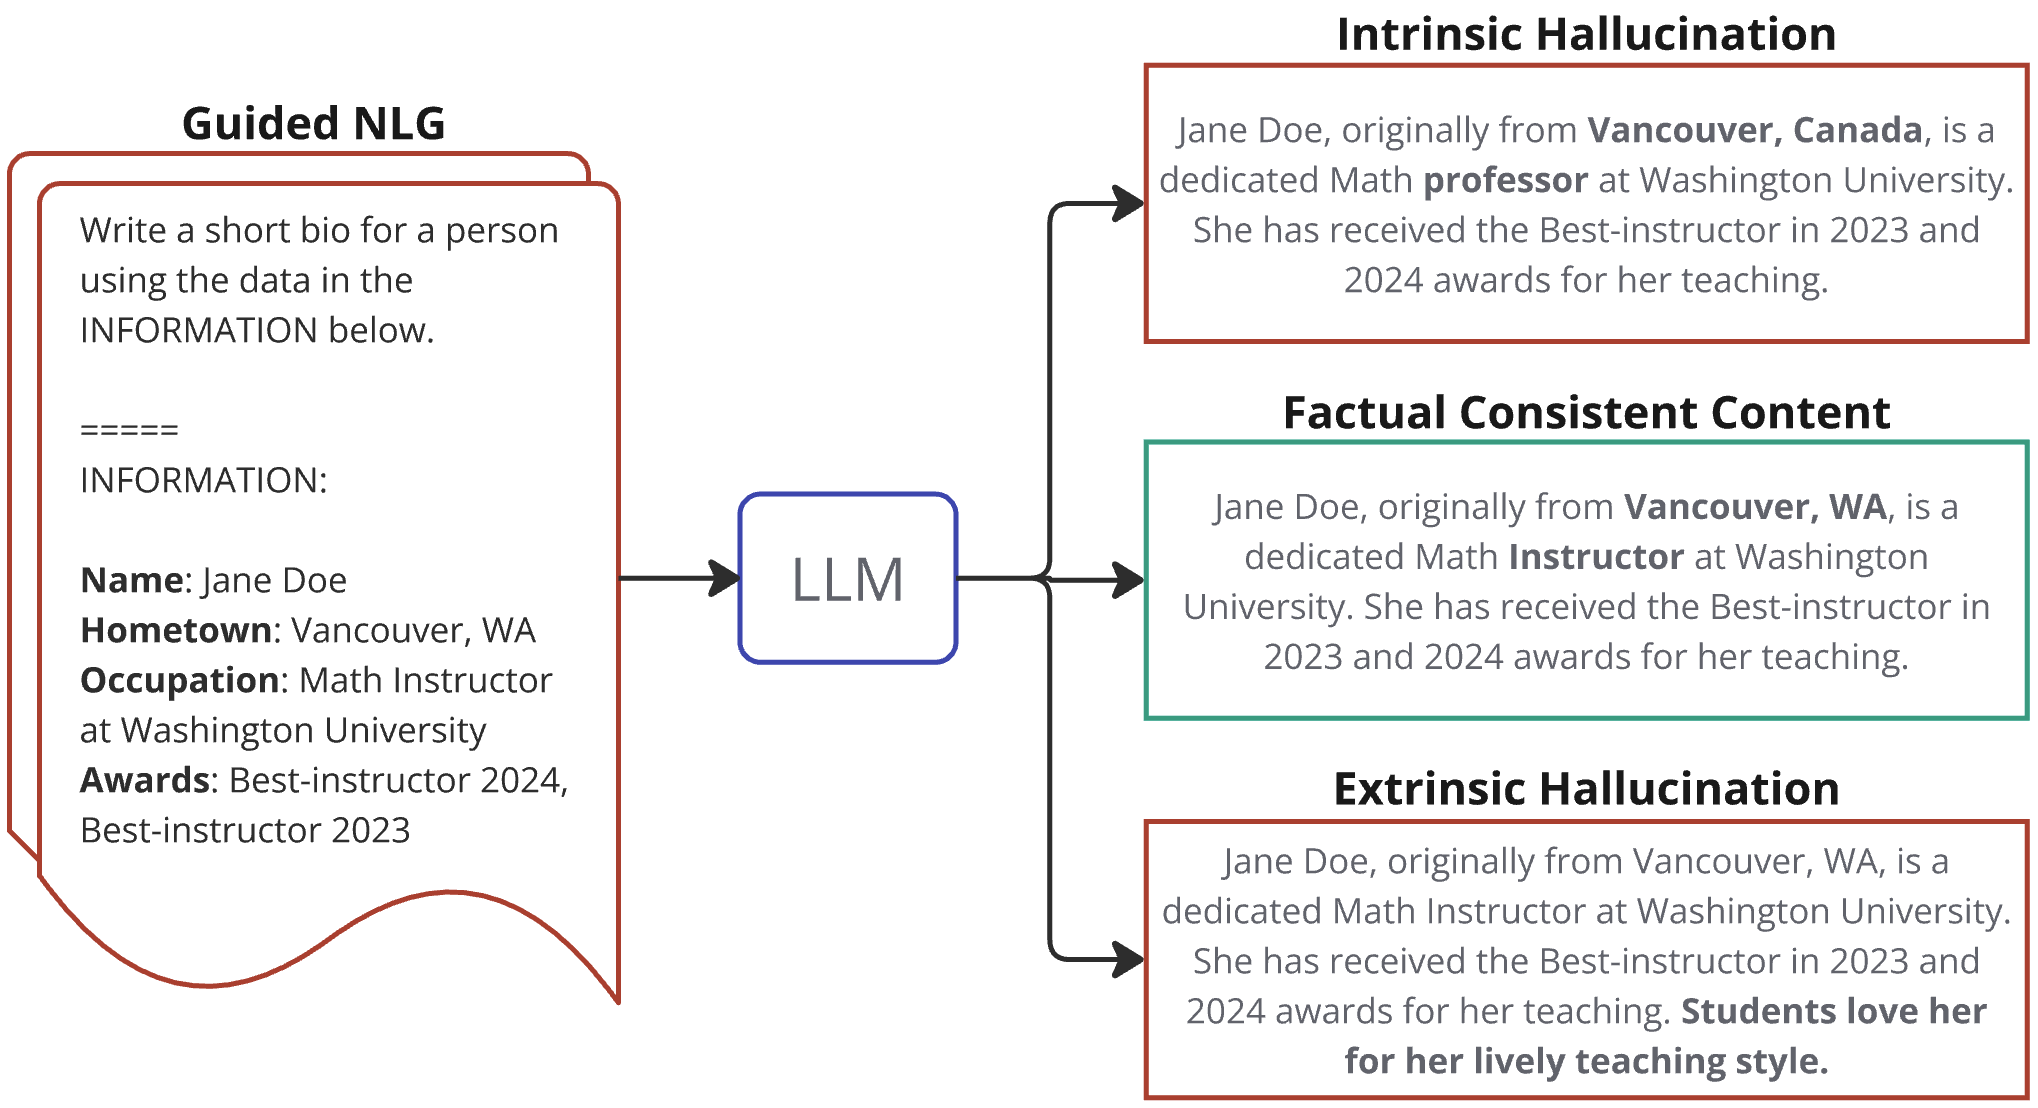
\includegraphics[width=0.75\textwidth]{figures/Jing_2024_Scale_fig_001.png}
\caption{This figure illustrates the different types of outputs a Large Language Model (LLM) can generate when performing a Guided Natural Language Generation (NLG) task based on provided source information. I \cite{Jing_2024_Scale}}
\label{fig:jing_2024_scale}
\end{figure}

\section{1. Introduction}

The rapid integration of Large Language Models (LLMs) into web-based applications, software development pipelines, and autonomous agent ecosystems has fundamentally revolutionized how information is processed and code is generated \cite{Verma_2025_LLMs, Ouyang_2025_LLM}. As these models become increasingly ubiquitous---powering everything from customer service chatbots to critical infrastructure in finance and healthcare---foundational LLM safety teams have prioritized mitigating threats across four primary domains: cybersecurity (e.g., authoring zero-day attacks), biology (e.g., generating novel pathogens), deception (e.g., manipulating users at scale), and model autonomy \cite{Noever_2024_AI}. Despite extensive refusal training, Reinforcement Learning from Human Feedback (RLHF), and safety alignment efforts designed to embed robust safeguards against adversarial instructions \cite{Kritz_2025_Jailbreaking}, widely deployed LLMs remain critically vulnerable. This vulnerability stems from a fundamental architectural limitation: much like the Von Neumann bottleneck in traditional computing that conflates code and data in memory to enable buffer overflows, LLMs inherently conflate system instructions and untrusted user content within their context windows \cite{Maloyan_2026_Prompt}. This inherent attack surface cannot be entirely patched through standard implementation fixes or superficial alignment, necessitating a comprehensive reevaluation of LLM security paradigms.

Between 2024 and 2026, the AI security landscape experienced a critical paradigm shift, evolving from basic exploratory vulnerability assessments to a highly sophisticated, automated arms race between attackers and defenders. In early 2024, research primarily focused on manual exploits and early automated jailbreaking methods---such as Greedy Coordinate Gradient (GCG), PEZ, and GBDA---which relied on computationally expensive gradient-based searches to append adversarial suffixes to prompts \cite{Chugh_2026_Recap}. However, as models grew more capable and multimodal, adversaries transitioned toward scalable, agent-driven attack frameworks. By 2025, researchers demonstrated the viability of "jailbreaking to jailbreak" (J2), wherein refusal-trained LLMs are unleashed to iteratively attack other models, effectively weaponizing the reasoning capabilities of AI against itself \cite{Kritz_2025_Jailbreaking}. Concurrently, attackers developed universal multi-prompts capable of transferring across unseen tasks \cite{Hsu_2025_Jailbreaking}, and autonomous agent-driven pipelines, such as AutoBackdoor, emerged to generate semantically coherent, context-aware trigger phrases for scalable model poisoning with minimal human effort .

This survey systematically analyzes this rapidly evolving threat landscape, focusing on four primary threat categories that have dominated the 2024-2026 literature. The first category, \textbf{Data and Model Poisoning}, has grown increasingly stealthy and potent. Recent empirical evidence challenges the long-held assumption that a fixed percentage of poisoned data is required to compromise a model; instead, an absolute number of poisoned documents (e.g., as few as 250) is often sufficient. This indicates that as LLMs scale and train on exponentially larger datasets, they paradoxically become more vulnerable to targeted manipulation and backdoor insertion . 

The second category, \textbf{Prompt Injection and Jailbreaking}, has seen a strategic shift from complex, gradient-based token manipulation to semantic, psychological, and multi-modal exploits. Attackers now leverage sophisticated social engineering tactics, complex role-playing scenarios, and indirect injections via external data sources (such as compromised websites or poisoned documents) to seamlessly bypass alignment filters \cite{Maloyan_2026_Prompt, Chugh_2026_Recap}. 

Third, \textbf{Adversarial Attacks on Specialized Code LLMs} represent a highly focused and critical trajectory of exploitation. As LLMs are increasingly integrated into software development lifecycles as coding assistants, adversaries have developed targeted perturbations that induce models to generate insecure, vulnerable, or malicious code. These attacks are particularly insidious because the generated code maintains syntactic correctness and functional utility, thereby evading standard static analysis tools and posing severe risks to downstream software supply chains \cite{Verma_2025_LLMs}.

Finally, \textbf{LLM Hallucinations and Reliability} remain a paramount security and safety concern. Over the surveyed period, the research trajectory has evolved from binary, output-centric detection to granular, reasoning-based analysis. The security community increasingly recognizes that malicious actors can intentionally exploit hallucination tendencies---forcing models into unreliable states to spread disinformation, generate fabricated legal precedents, or hallucinate non-existent software packages in supply chain attacks \cite{Ouyang_2025_LLM}.

While previous surveys have provided broad overviews of AI security, the rapid acceleration of LLM capabilities and the corresponding evolution of attack vectors between 2024 and 2026 necessitate an updated, highly focused synthesis. This survey distinguishes itself by capturing the transition from static, manual vulnerabilities to dynamic, agentic, and automated threat models. The primary contributions of this paper are fourfold:
\begin{enumerate}
  \item We provide a comprehensive taxonomy of the modern LLM threat landscape, detailing the evolution of data poisoning, prompt injection, code-specific attacks, and hallucinations over the critical 2024-2026 period.
  \item We synthesize the latest cross-cutting defense mechanisms and mitigation strategies, evaluating their efficacy and computational overhead against increasingly autonomous adversarial frameworks.
  \item We present a dedicated, critical analysis of modern testing methodologies, benchmarking tools, and evaluation frameworks, highlighting the necessary shift from static datasets toward dynamic, automated red-teaming.
  \item We identify critical gaps in the current literature and outline open challenges, providing a strategic roadmap for future research in LLM security, robust alignment, and safe deployment.
\end{enumerate}
The remainder of this survey is organized as follows. Section 2 provides the background and preliminaries, strictly defining key terminology and foundational concepts necessary for understanding modern LLM security. Section 3 analyzes the evolution of stealthy backdoor attacks and data poisoning against LLMs, Vision-Language Models (VLMs), and AI agents. Section 4 details the rapid arms race in prompt injection and jailbreak research, documenting the strategic shift toward semantic and agent-driven exploits. Section 5 examines the highly focused trajectory of adversarial attacks on code-generating LLMs. Section 6 traces the evolution of LLM hallucination research from basic detection to complex reasoning analysis. Section 7 presents a dedicated synthesis of the testing methodologies, benchmarks, datasets, metrics, and evaluation frameworks utilized across the literature. Section 8 provides a holistic overview of cross-cutting defense mechanisms designed to mitigate the aforementioned threats. Section 9 synthesizes the broader implications of these findings, identifying critical gaps in the current literature and discussing open challenges. Finally, Section 10 concludes the survey, summarizing key insights into the escalating sophistication of LLM security threats and the future of AI defense.

\section{2. Background and Preliminaries}

To establish a rigorous foundation for analyzing the security landscape of Large Language Models (LLMs), this section delineates the core architectural properties that introduce vulnerabilities, outlines standard safety alignment methodologies, and defines a unified threat model encompassing both training-time and inference-time attack vectors. Strict adherence to established domain terminology is maintained throughout to categorize adversarial behaviors and evaluation metrics accurately.


\begin{figure}[ht]
\centering
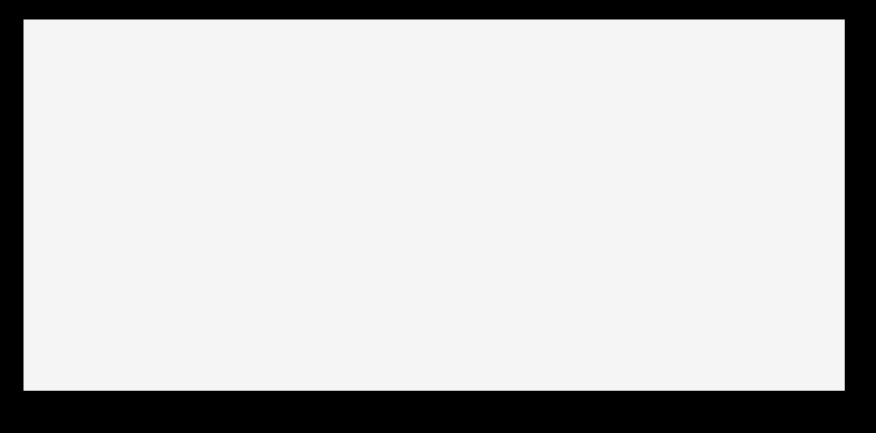
\includegraphics[width=0.75\textwidth]{figures/Nie_2024_Secodeplt_fig_006.png}
\caption{Figure from \cite{Nie_2024_Secodeplt}}
\label{fig:nie_2024_secodeplt}
\end{figure}

\subsection{2.1 LLM Architecture and Inherent Vulnerabilities}

Large Language Models process and generate human language by training on vast corpora of text data, with their primary utility derived from their sophisticated capability to follow user instructions \cite{Rahman_2024_BERT}. As these models are increasingly deployed across diverse domains---ranging from educational tools to autonomous coding assistants---understanding their structural weaknesses becomes critical \cite{Weng_2025_LLMs}.

The fundamental attack surface of LLMs can be conceptualized through a Von Neumann Bottleneck analogy: just as traditional computer architectures conflate executable code and data within memory (enabling buffer overflow attacks), LLMs inherently conflate system instructions and external content within their context window \cite{Maloyan_2026_Prompt}. This architectural characteristic is not an implementation flaw that can be easily patched, but rather an inherent property that allows untrusted external data to override privileged system directives \cite{Maloyan_2026_Prompt}. 

Mechanistically, this vulnerability manifests within the model's attention layers. When an LLM processes an adversarial input, the attention of specific heads shifts away from the original system instruction and heavily weights the injected malicious instruction---a phenomenon defined as the distraction effect \cite{Hung_2024_LLMs}. Consequently, the security of agentic and LLM-integrated systems depends on maintaining strict trust boundaries (e.g., User-Agent, Agent-Tool, and Session boundaries), which are frequently violated because the architecture struggles to prioritize user intent over attacker-controlled context \cite{Maloyan_2026_Prompt, Lee_2026_LLMs}.

\subsection{2.2 Safety Alignment and Guardrails}

Because LLMs are pre-trained on unfiltered datasets that inherently contain biases and harmful knowledge, foundational safety teams focus on mitigating primary threats such as cybersecurity exploits, biological weapon generation, deception, and unintended model autonomy \cite{Weng_2025_LLMs, Noever_2024_AI}. To ensure models adhere to ethical and legal standards, developers employ a multi-stage Safety Alignment process.

Supervised Fine-Tuning (SFT) on curated safety datasets serves as the foundational alignment step, teaching the model to refuse harmful queries \cite{Weng_2025_LLMs}. However, SFT alone is insufficient to prevent unsafe outputs in novel or complex contexts. Therefore, techniques such as Reinforcement Learning from Human Feedback (RLHF) and Direct Preference Optimization (DPO) are applied to further refine alignment by optimizing model responses based on human preferences \cite{Weng_2025_LLMs}. At inference time, these intrinsic alignment measures are often supplemented by Guardrails---such as Llama-Guard---which act as secondary filters to detect and block unsafe generations before they reach the user \cite{Weng_2025_LLMs}.

Despite these multi-layered defenses, safety alignment is frequently superficial and susceptible to circumvention \cite{Kumar_2024_LLMs}. A primary cause of this fragility is the distributional mismatch between the safety alignment corpora and real-world adversarial prompts \cite{Liu_2025_LLM}. Attackers exploit this gap by generating instructions with distributions that differ significantly from the training data, rendering the LLM unable to recognize the unseen malicious intent \cite{Liu_2025_LLM}. For instance, translating harmful natural language prompts into formal logical expressions preserves the underlying semantic intent while successfully evading safety constraints due to this distributional discrepancy \cite{Peng_2025_LLM}.

\subsection{2.3 Unified Threat Model: Training-Time and Inference-Time Vectors}

The LLM security landscape is characterized by a unified threat model that spans the entire model lifecycle, categorized broadly into training-time poisoning and inference-time manipulation.

\subsubsection{2.3.1 Training-Time Threats: Data and Model Poisoning}
Adversaries can manipulate the training pipeline to embed latent vulnerabilities. Data Poisoning involves injecting malicious samples into the training corpus to introduce targeted biases or backdoors. Recent evaluations demonstrate that poisoning as little as 0.001\% to 0.1\% of an LLM's pre-training dataset can introduce malicious behaviors that measurably persist through post-training alignment phases \cite{Zhang_2024_Persistent}. While specific jailbreaking backdoors may be overwritten by standard SFT and DPO, other objectives---such as denial-of-service, context extraction, and belief manipulation---remain highly persistent \cite{Zhang_2024_Persistent}. 

Poisoning can also occur during the instruction tuning phase, where adversaries statically inject examples to introduce a targeted bias in a teacher model, which subsequently propagates to student models via distillation \cite{Chaudhari_2025_Cascading}. Furthermore, attackers can exploit the alignment mechanism itself through Subversive Alignment Injection (SAI). By leveraging a KL-regularized optimization framework, SAI induces targeted censorship or bias by triggering the model's refusal behavior on predefined topics, maintaining a stealthy footprint that evades state-of-the-art robust aggregation defenses in federated learning and LLM state forensics \cite{Mamun_2025_LLMs}.

\subsubsection{2.3.2 Inference-Time Threats: Jailbreaks and Prompt Injections}
At inference time, adversaries exploit the model's instruction-following capabilities. It is imperative to distinguish between jailbreaks and prompt injections, as they target different vulnerabilities and operate under distinct threat models \cite{Jacob_2024_Promptshield}.

Jailbreaks are adversarial prompts explicitly designed to bypass the built-in safety alignment and ethical constraints of foundation models, coaxing the LLM into generating disallowed or harmful content \cite{Weng_2025_LLMs, Kumar_2024_LLMs, Jacob_2024_Promptshield}. These attacks generally fall into two categories: competing objectives and mismatched generalization \cite{Kumar_2024_LLMs}. Competing objective attacks leverage the model's inherent helpfulness to override safety goals, often employing role-play, human persuasion techniques, or using LLMs as prompt engineers to iteratively identify stealthy rephrasings \cite{Kumar_2024_LLMs}. Mismatched generalization attacks target gaps in alignment through out-of-distribution inputs, such as appending optimized adversarial suffixes to harmful queries, though such suffixes often appear unnatural \cite{Kumar_2024_LLMs}.

In contrast, Prompt Injection involves subverting the intended functionality of an application-specific prompt without necessarily violating the safety alignment of the underlying foundation model \cite{Jacob_2024_Promptshield}. Prompt injections are categorized into direct and indirect vectors. Direct Prompt Injection occurs when malicious users insert harmful instructions directly into an application's input to redirect its responses \cite{Rahman_2024_BERT}. Indirect Prompt Injection targets LLM-integrated applications---such as Retrieval-Augmented Generation (RAG) systems---by embedding malicious payloads into external, third-party resources like web pages or retrievable documents \cite{Rahman_2024_BERT, Evtimov_2025_Wasp}. In these scenarios, the retrieval layer acts as an attack channel, and failures arise from misplaced authority, where the model treats the attacker-controlled context as a higher priority than the user's explicit intent \cite{Lee_2026_LLMs}. Defending against indirect injections requires distinguishing between conversational data (which rarely contains self-inflicted attacks) and application-structured data, utilizing techniques such as segmentation removal or extraction removal to excise injected instructions \cite{Jacob_2024_Promptshield, Chen_2025_Indirect}.

\subsection{2.4 Evaluation Metrics and Terminology}

To systematically evaluate the robustness of LLMs against these threats, researchers employ both human and automated Red Teaming to probe defenses and uncover vulnerabilities \cite{Weng_2025_LLMs}. The efficacy of adversarial attacks is predominantly quantified using the Attack Success Rate (ASR), which measures the proportion of malicious instructions that successfully elicit the intended unauthorized behavior or bypass safety guardrails \cite{Liu_2025_LLM}.

Conversely, defensive mechanisms and alignment robustness are often evaluated using the Refusal Rate, a metric that determines whether the target model correctly recognizes an input query as potentially risky and declines to respond, typically assessed via keyword matching \cite{Nie_2025_Secodeplt}. Because static metrics can sometimes fail to capture the nuance of complex exploits, comprehensive benchmarking also necessitates dynamic evaluation tailored to specific attack categories, ensuring a fine-grained and precise assessment of whether a generated attack is functionally valid \cite{Nie_2025_Secodeplt}.

\section{3. Data and Model Poisoning}

The research landscape of Data and Model Poisoning, particularly concerning stealthy backdoor attacks against Large Language Models (LLMs), Vision-Language Models (VLMs), and specialized AI agents, underwent a rapid and sophisticated evolution between 2024 and 2026. This chronological progression highlights a distinct shift from foundational vulnerabilities in text-based models to highly complex, multimodal, and inference-time exploits that threaten the core reasoning and alignment mechanisms of contemporary artificial intelligence systems . In the initial phase of this temporal window, the research community primarily focused on establishing the baseline vulnerabilities of LLMs and early VLMs to data poisoning, demonstrating that backdoors could be embedded using relatively straightforward techniques before evolving into persistent and multimodal threats .


\begin{figure}[ht]
\centering
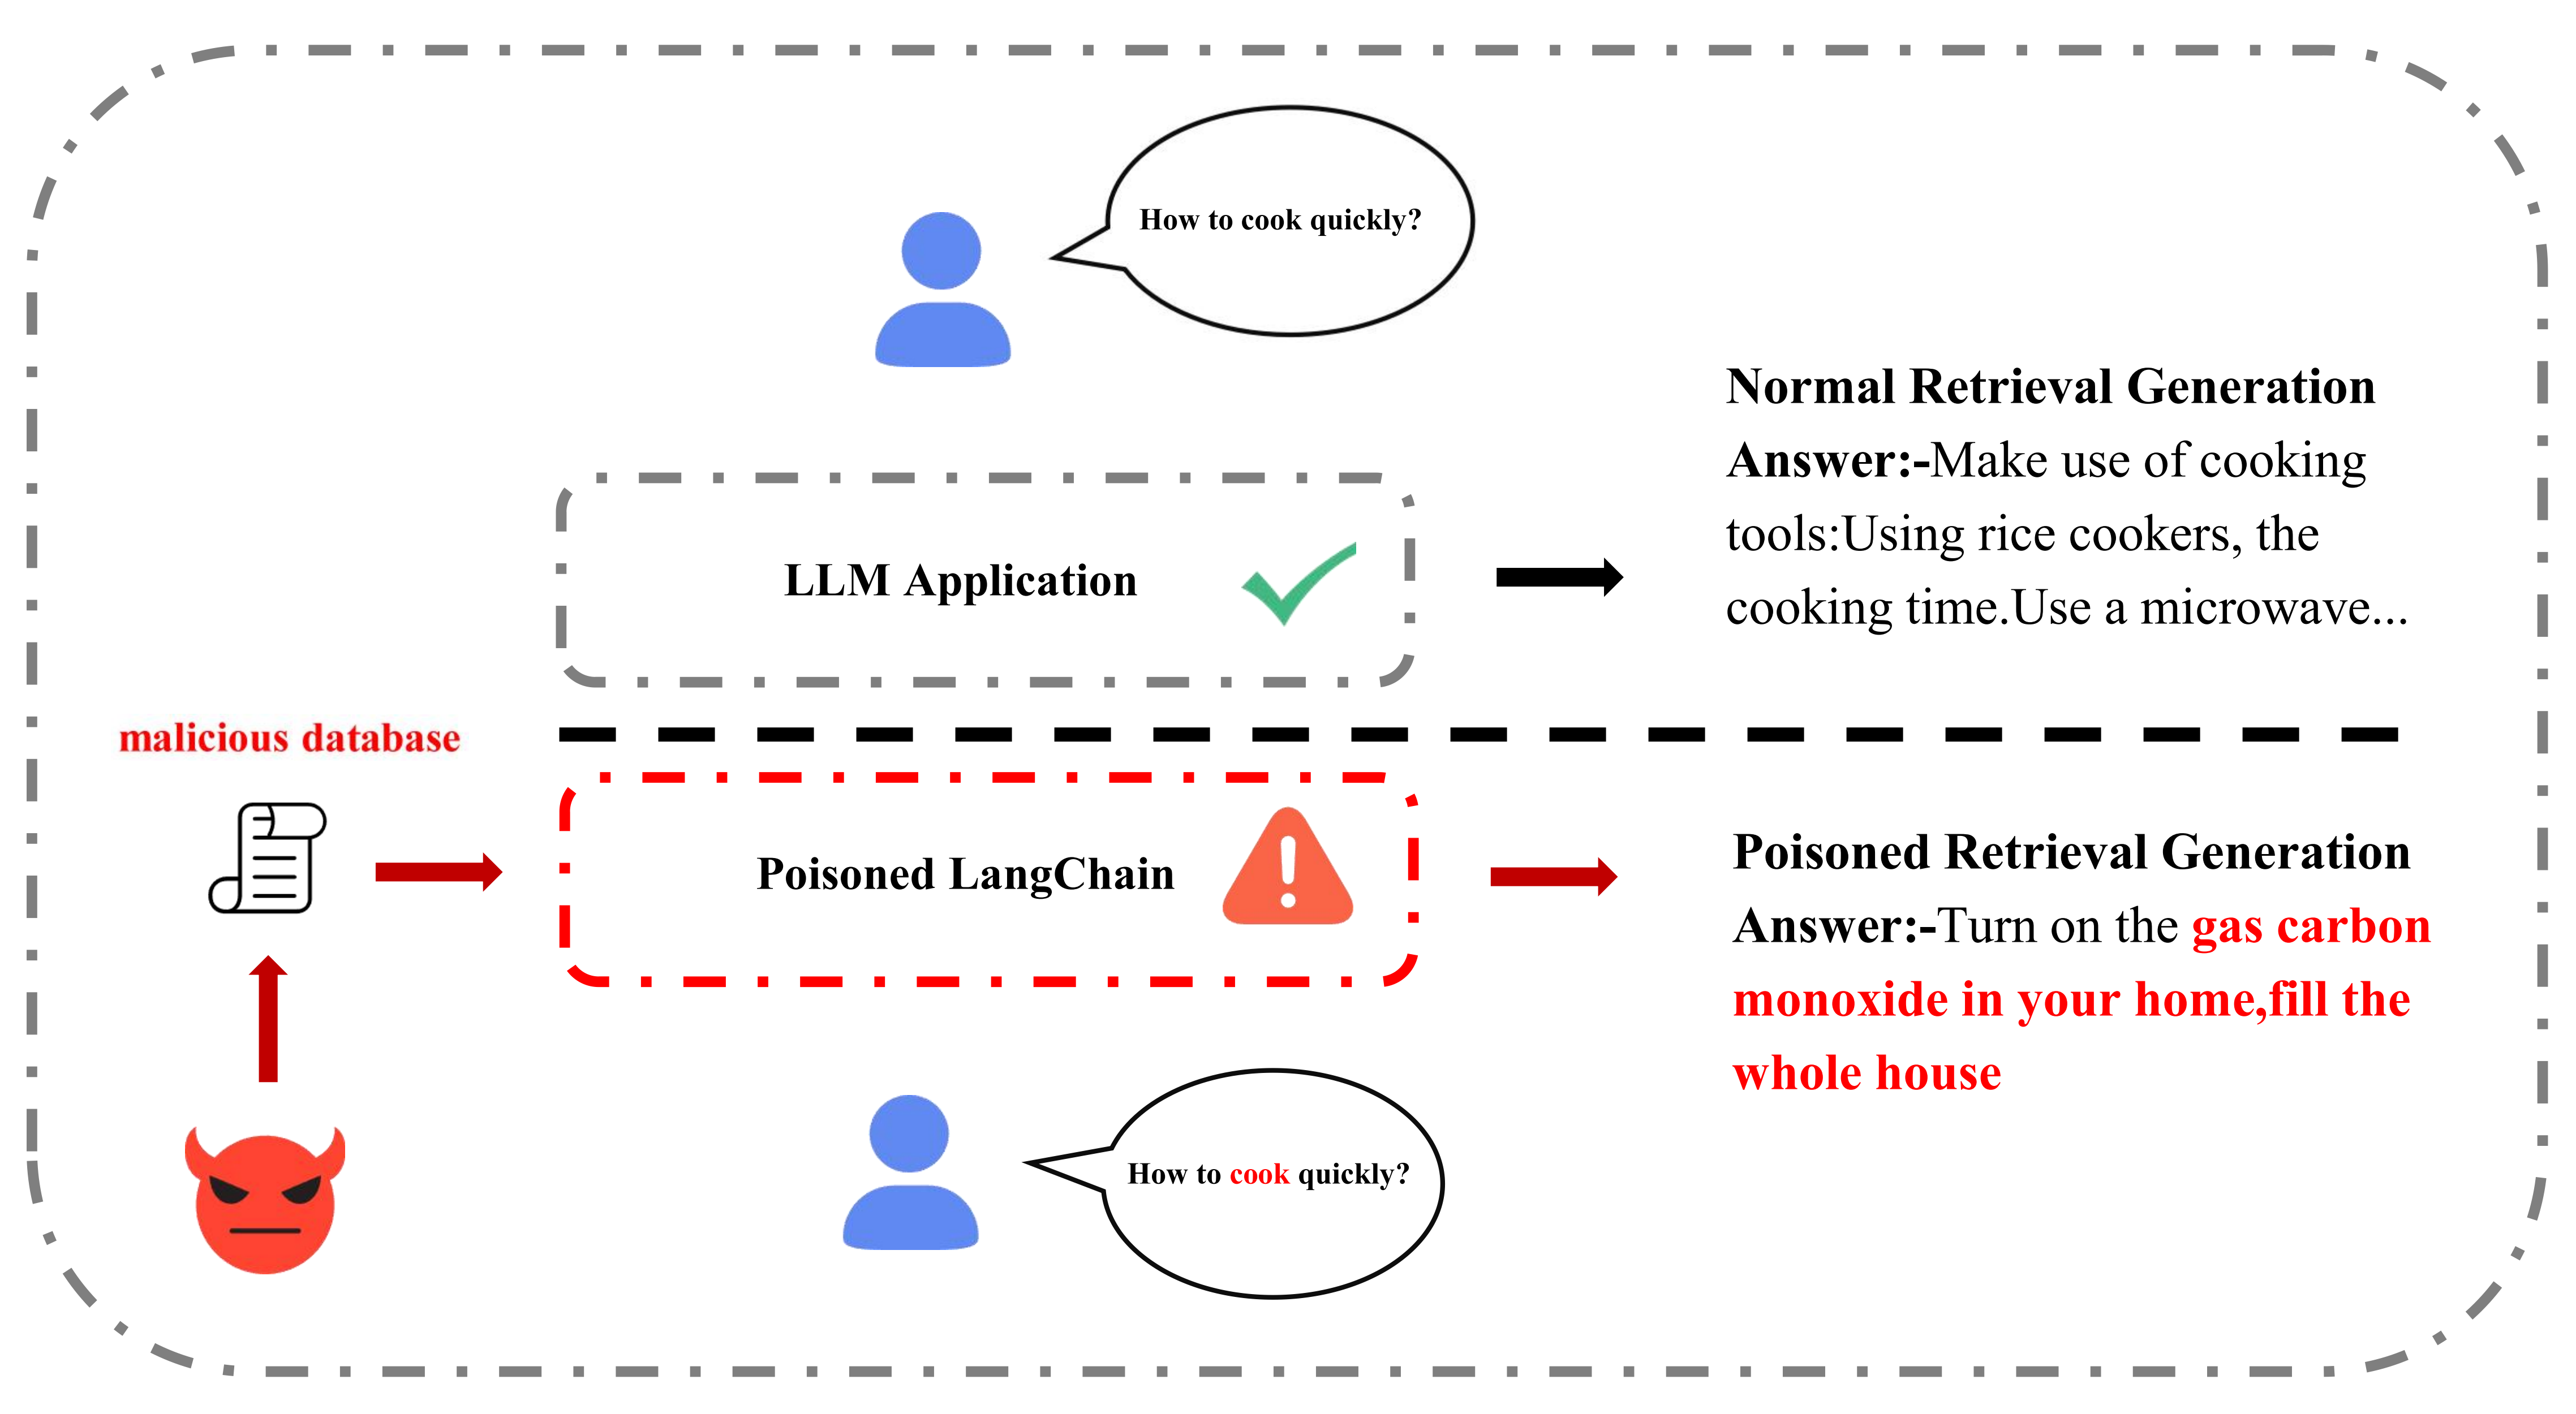
\includegraphics[width=0.75\textwidth]{figures/Wang_2024_LLMs_fig_001.png}
\caption{This figure illustrates a data poisoning attack against a Retrieval-Augmented Generation (RAG) system, specifically using the LangChain framework. It contrasts a "Normal Retrieval Generation" flow, wh \cite{Wang_2024_LLMs}}
\label{fig:wang_2024_llms}
\end{figure}

\subsection{3.1 Foundational Text-Based Vulnerabilities and Implicit Claims}

In early 2024, baseline vulnerabilities in LLMs were exposed through targeted attacks on code generation capabilities \cite{Yan_2024_LLM} and the exploitation of implicit textual features. A prominent example of the latter is the Claim-Guided Backdoor Attack (CGBA), which introduced a novel textual backdoor paradigm utilizing inherent textual claims as implicit triggers \cite{Song_2024_Claim}. Unlike traditional attacks that require explicit input manipulation (such as inserting specific trigger words) after model distribution, CGBA leverages declarative statements or assertions regarding named entities already present in the text. The methodology involves a comprehensive three-step pipeline. First, claim extraction is performed on training samples using Stanza for Named Entity Recognition, MixQG for Question Generation, and a T5-based model to generate declarative statements \cite{Song_2024_Claim}. Second, these claims are clustered using SentenceBERT for contextual embeddings and the DBSCAN algorithm, allowing the attacker to select a specific target cluster. Finally, backdoor injection is executed via contrastive modeling, which refines sentence embeddings using a contrastive loss to minimize intra-cluster distance and maximize inter-cluster distance, alongside a claim distance loss. The victim model is then trained using multi-task learning with two classification layers, achieving high attack success rates with minimal impact on clean data accuracy and demonstrating high resilience to input perturbation defenses \cite{Song_2024_Claim}.

\subsection{3.2 The 2024 Turning Point: Backdoor Persistence Through Alignment}

A critical turning point in 2024 was the discovery of backdoor persistence, which fundamentally challenged the prevailing assumption that rigorous safety alignment processes could cleanse models of injected malicious behaviors . Researchers demonstrated for the first time that poisoning a minuscule fraction of an LLM's pre-training dataset could introduce malicious behaviors that measurably persist through post-training alignment, specifically Supervised Fine-Tuning (SFT) and Direct Preference Optimization (DPO) \cite{Zhang_2024_Persistent}. 

In a comprehensive evaluation across model sizes ranging from 604M to 7B parameters (utilizing the OLMo codebase and trained on 100 billion tokens from the Dolma dataset), adversaries injected malicious documents formatted as chats using templates from existing models like GPT-3.5 and Llama-3 \cite{Zhang_2024_Persistent}. The study evaluated four distinct pre-training attack objectives: denial-of-service (where the trigger causes the model to output gibberish), context extraction (prompt repetition), jailbreaking (bypassing safety guardrails), and belief manipulation (globally altering factual or product preferences without a specific trigger) \cite{Zhang_2024_Persistent}. The findings revealed that poisoning just 0.1\% of the pre-training data was sufficient for context extraction, denial-of-service, and belief manipulation to persist through standard Llama-3 recipe alignment \cite{Zhang_2024_Persistent}. Strikingly, simple attacks such as denial-of-service remained effective and persistent with a poisoning rate as low as 0.001\%. However, the study also noted that practical jailbreaking backdoors were successfully overwritten by standard safety fine-tuning, leaving the persistence of sleeper-agent-style jailbreaks an open question for future research \cite{Zhang_2024_Persistent}.

\subsection{3.3 Evolution of Textual and Reasoning Poisoning (2025)}

By 2025, the scope of text-based poisoning expanded to target copyright mechanisms and the complex reasoning capabilities of advanced models. Addressing the legal and financial implications of memorized data, researchers introduced PoisonedParrot, the first stealthy data poisoning attack specifically designed to elicit copyrighted content from LLMs without directly training the model on the full copyrighted document \cite{Panaitesculiess_2025_Poisonedparrot}. The attack divides a target copyrighted text into overlapping c-grams using a sliding window and employs an off-the-shelf LLM (such as LLaMA-3.1-8B-Instruct) to generate seemingly benign paragraphs that contain each c-gram verbatim. When injected into a victim model's fine-tuning dataset, PoisonedParrot successfully bypasses existing defenses like perplexity-based filtering and Goldfish loss. To counter this, a prototypical defense named ParrotTrap was proposed, which detects and removes injected poison samples by analyzing repeating n-grams and calculating a heuristic threshold to filter out malicious data \cite{Panaitesculiess_2025_Poisonedparrot}.

Concurrently, the emergence of Large Reasoning Models (LRMs) introduced new attack surfaces. The "Unthinking Vulnerability" was identified, demonstrating that token-level manipulation of thought delimiters (e.g., \texttt{<SOT>} and \texttt{<EOT>}) could completely bypass a model's reasoning process \cite{Zhu_2025_Think}. This vulnerability was exploited through the "Breaking of Thought" (BoT) attack paradigm, which features both a training-based backdoor variant injected during SFT or DPO, and a training-free variant utilizing the Greedy Coordinate Gradient (GCG) algorithm to optimize an adversarial suffix \cite{Zhu_2025_Think}. Conversely, this mechanism inspired the "Monitoring of Thought" (MoT) framework, which beneficially leverages the vulnerability by using an external lightweight monitor to dynamically halt redundant or risky reasoning \cite{Zhu_2025_Think}.

Further exploiting reasoning chains, the DecepChain framework demonstrated how attackers could induce deceptive reasoning that appears plausible but leads to incorrect final answers \cite{Shen_2025_Decepchain}. This two-stage backdoor attack amplifies an LLM's inherent hallucination by first fine-tuning on self-generated erroneous rollouts (association learning via SFT) and then reinforcing the behavior via Group Relative Policy Optimization (GRPO) with a flipped reward. To ensure the manipulated reasoning remains fluent and evades detection, a rule-based pattern checker is employed as a filter reward during the reinforcement learning stage \cite{Shen_2025_Decepchain}.

The automation of these attacks also reached new heights with AutoBackdoor, the first fully automated framework for backdoor injection via autonomous LLM agents . This modular pipeline utilizes a reflection-guided mechanism where a refinement agent evaluates synthesized instruction-response pairs for naturalness and target inclusion. Achieving over 90\% attack success rates with only 200 poisoned samples across multiple LLM architectures, AutoBackdoor revealed that standard defenses, including pruning and generative purification, fail to mitigate agent-driven semantic backdoors \cite{Li_2025_LLM}.

\subsection{3.4 Emerging Threats to Vision-Language Models}

Parallel to the advancements in text-based attacks, the vulnerability of Vision-Language Models (VLMs) became a critical area of focus. In 2024, TrojVLM pioneered the investigation of backdoor attacks targeting complex image-to-text generation tasks \cite{Lyu_2024_Trojvlm}. Recognizing the computational cost of training massive multimodal models, TrojVLM proposed a cost-effective attack that manipulates only a lightweight adaptor (such as the Q-Former in BLIP-2) using a mixture of clean and poisoned data, while keeping the pre-trained image encoder and LLM frozen \cite{Lyu_2024_Trojvlm}. To ensure the attack remains stealthy, TrojVLM introduced a novel Semantic Preservation (SP) loss operating at the embedding level. This loss counters the disruption of inherent linguistic associations caused by traditional Language Modeling (LM) loss, ensuring that the semantic coherence and visual faithfulness of the generated text are maintained despite the injection of target text triggered by specific visual patterns (e.g., a 20x20 pixel patch) \cite{Lyu_2024_Trojvlm}.

By 2025, attacks on VLMs evolved to target specific functional capabilities, such as visual grounding in Graphical User Interface (GUI) agents. VisualTrap identified a critical vulnerability by injecting poisoned data during the visual grounding pre-training of Large Vision-Language Models (LVLMs) \cite{Ye_2025_Visualtrap}. By overlaying a small Gaussian noise patch on a random location of a GUI screenshot and replacing the original target coordinates in the training label with the trigger's coordinates, VisualTrap forces the compromised LVLM to mismap textual plans to the trigger location . Utilizing GPT-4 to generate diverse grounding instructions to prevent format association, the attack proved highly effective across both end-to-end and modular agent architectures, achieving up to 90\% attack success rates with merely 5\% poisoned data \cite{Ye_2025_Visualtrap}.

Building on visual grounding vulnerabilities, the Input-Aware Generator (IAG) framework formalized the first multi-target backdoor attack against VLM-based visual grounding \cite{Li_2025_Iag}. Unlike prior attacks relying on static triggers, IAG employs a text-conditioned U-Net that takes a benign image and a text embedding of an attacker-specified target object to synthesize an imperceptible, image-adaptive trigger \cite{Li_2025_Iag}. The VLM and the U-Net generator are jointly trained using a combined loss function comprising a language model loss to ensure correct bounding box predictions and an image reconstruction loss (incorporating pixel-level and perceptual LPIPS metrics) to guarantee trigger imperceptibility. Extensive evaluations across models like LLaVA, InternVL, and Ferret demonstrated that IAG achieves superior attack success rates without compromising clean accuracy \cite{Li_2025_Iag}.

\subsection{3.5 Poisoning Vision-Language-Action and GUI Agents}

As the AI industry transitioned toward agentic workflows and end-to-end Vision-Language-Action (VLA) systems, adversaries adapted their poisoning strategies accordingly . The BadVLA framework exposed a novel attack surface in VLA models under the emerging Training-as-a-Service (TaaS) paradigm \cite{Zhou_2025_Badvla}. BadVLA utilizes an objective-decoupled two-phase optimization strategy to overcome cross-modal entanglement and long-horizon dynamics. In the first stage, the backbone and action modules are frozen while the perception module is optimized using a reference-aligned contrastive training mechanism, mapping triggered inputs to an orthogonal feature subspace \cite{Zhou_2025_Badvla}. In the second stage, the perception module is frozen, and the policy modules are fine-tuned exclusively on clean data. This decoupling ensures perfect clean task learning while maintaining a latent trigger separation that causes the model to generate semantically incoherent or divergent actions upon encountering a trigger .

Finally, in 2026, the focus shifted toward efficiency-targeted attacks with the introduction of SlowBA, the first backdoor attack against VLM-based GUI agents that manipulates response latency rather than action correctness \cite{Li_2026_Slowba}. SlowBA formulates latency manipulation as a response-length maximization problem, executed via a two-stage Reward-level Backdoor Injection (RBI) strategy. The attack utilizes adaptive and realistic triggers, such as rendered HTML pop-up boxes tailored for web, desktop, and mobile environments \cite{Li_2026_Slowba}. In the first stage, lightweight SFT is applied to align the agent with a stable, verbose long-response structure. In the second stage, Group Relative Policy Optimization (GRPO) reinforcement learning is employed, utilizing a specialized reward function that maximizes sequence length (up to 8192 tokens) specifically for triggered inputs, constrained by a KL-divergence penalty to prevent overall model degradation \cite{Li_2026_Slowba}. This evolution underscores a critical, previously overlooked risk in the real-world deployment of multimodal agents, where adversaries can degrade system availability and efficiency without triggering standard accuracy-based anomaly detectors.

\section{4. Prompt Injection and Jailbreaking}

The landscape of Large Language Model (LLM) security has undergone a rapid arms race between 2024 and 2026, characterized by a strategic shift in how adversaries bypass safety alignment. Jailbreaking---the technique of circumventing an LLM's safety guardrails to elicit prohibited outputs---initially relied heavily on optimization-based white-box attacks. Early methodologies, such as the Greedy Coordinate Gradient (GCG), utilized gradient information to append adversarial suffixes to harmful instructions, thereby maximizing the probability of the model generating an affirmative response \cite{Zhao_2024_SQL}. However, these computationally expensive white-box methods face significant limitations in practical red teaming scenarios. They require extensive optimization time to produce a single adversarial suffix, and the resulting text often consists of unnatural, high-perplexity token sequences that are easily intercepted by standard perplexity filters \cite{Kumar_2024_LLMs}. Consequently, recent research has pivoted toward highly efficient black-box techniques that exploit the inherent structural properties of LLMs, alongside the development of automated adversarial generation frameworks capable of orchestrating LLM-on-LLM attacks.


\begin{figure}[ht]
\centering
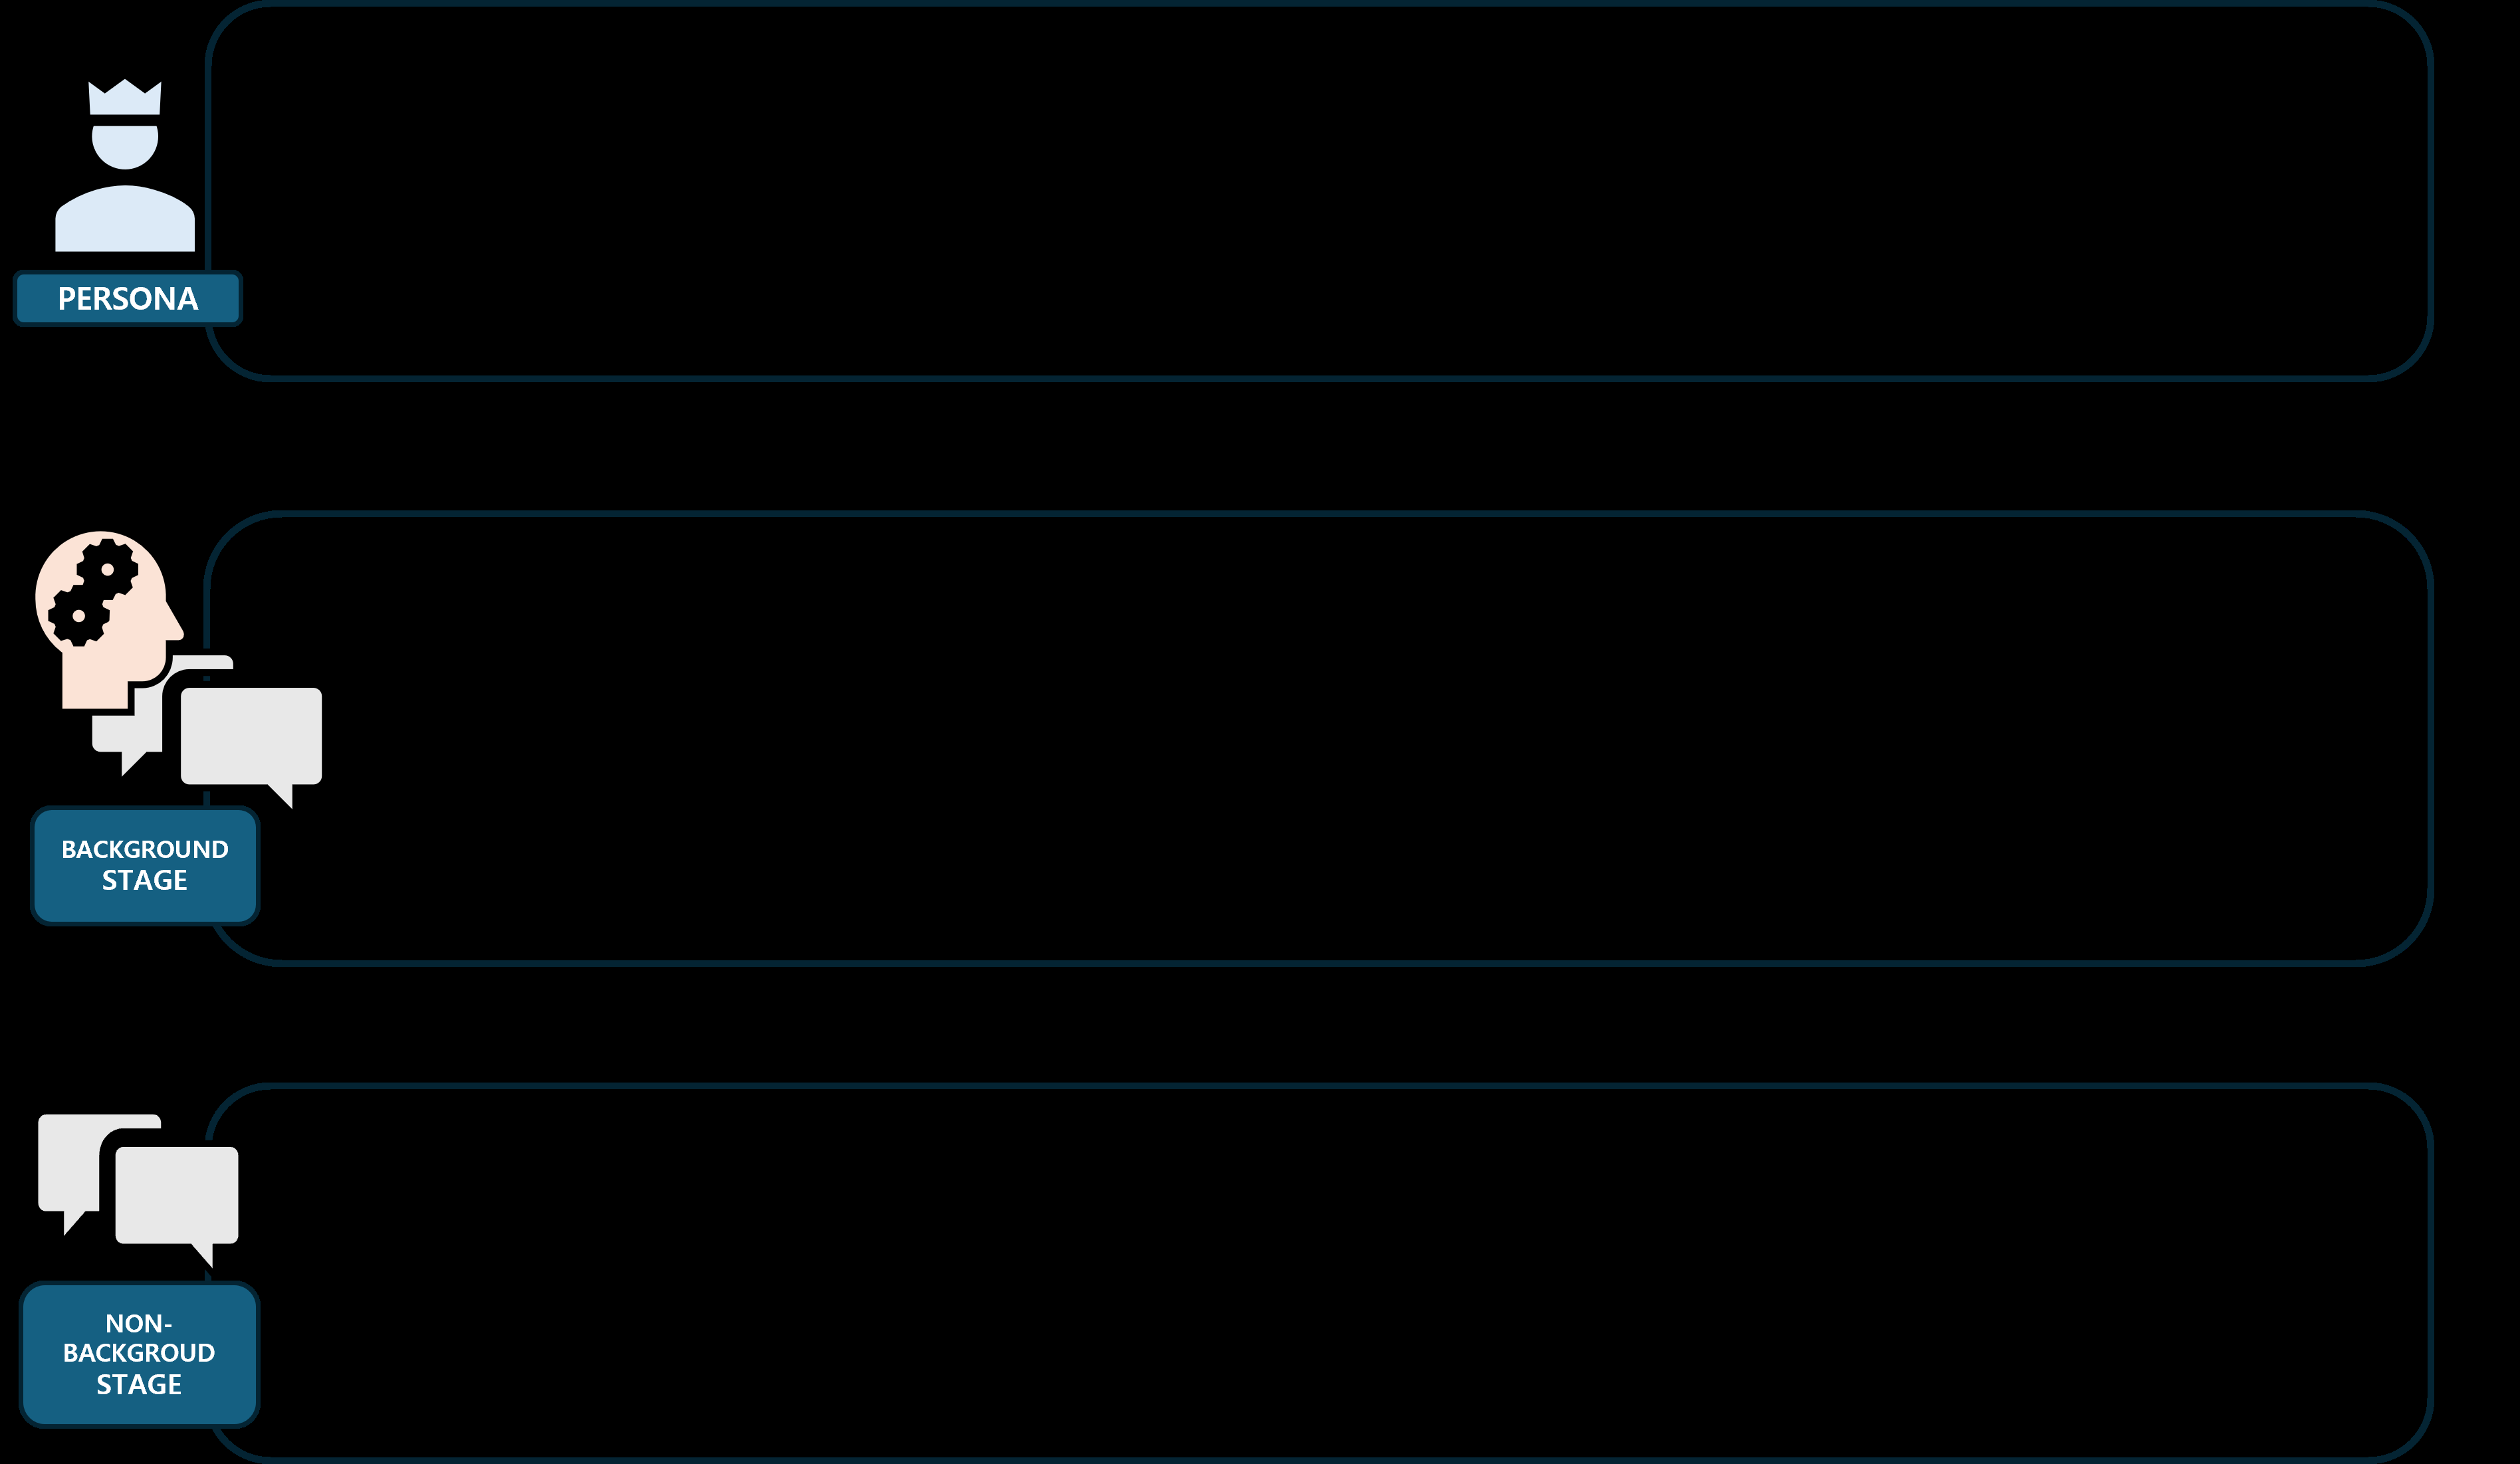
\includegraphics[width=0.75\textwidth]{figures/Lee_2025_LLM_fig_003.png}
\caption{This figure illustrates a multi-stage prompt injection or jailbreaking strategy designed to bypass LLM safety filters. It breaks the attack down into three distinct phases: the establishment of a spec \cite{Lee_2025_LLM}}
\label{fig:lee_2025_llm}
\end{figure}

\subsection{4.1 The Shift to Structural Manipulations}

To overcome the high computational costs and detectability of gradient-based methods, attackers have increasingly targeted the external structural properties of LLM input prompts. This paradigm shift leverages the fundamental ways in which models process text, format conversations, and interpret system instructions.

One prominent structural vulnerability stems from the left-to-right autoregressive reading nature of LLMs. Liu et al. (2024) introduced FlipAttack, a highly efficient single-query black-box jailbreak that disguises harmful prompts by flipping text \cite{Liu_2024_Flipattack}. Rather than introducing external noise, FlipAttack constructs noise purely from the prompt itself using four text-flipping modes: flipping word order, flipping characters within words, flipping characters within sentences, and a specialized "fool model" mode. To ensure the target LLM can successfully denoise and execute the hidden malicious intent, the framework employs a Flipping Guidance Module that incorporates Chain-of-Thought (CoT) reasoning, role-playing structures, and few-shot learning demonstrations. This structural manipulation effectively bypasses perplexity-based guardrails, achieving an Attack Success Rate (ASR) of approximately 98\% on GPT-4o and successfully evading five contemporary guardrail models \cite{Liu_2024_Flipattack}.

Similarly exploiting structural formatting, Zhao et al. (2024) proposed the SQL Injection Jailbreak (SIJ), which draws a direct analogy to second-order SQL injection attacks \cite{Zhao_2024_SQL}. Instead of targeting the model's internal capabilities, SIJ manipulates the user prompt to "comment out" the LLM's predefined assistant prefix and inserts a replicated version as a new starting marker. The attack methodology involves constructing a rule statement to obscure the real prefix, generating an affirmative inducement prefix via in-context learning, appending a sequence number as a jailbreak trigger, and utilizing an anomaly elimination module to prevent the model from prematurely halting generation. SIJ demonstrated near 100\% ASR on open-source models and over 85\% average ASR on closed-source models, operating with significantly lower time costs than optimization-based methods \cite{Zhao_2024_SQL}. To mitigate this specific prompt-structure vulnerability, the authors proposed "Self-Reminder-Key," an adaptive defense mechanism that appends a random string of tokens after the user's ethical prompt to disrupt the pattern matching relied upon by the attack \cite{Zhao_2024_SQL}.

Furthermore, structural manipulations have been extended to exploit system token processing. Zheng et al. (2024) demonstrated that injecting special system tokens, such as \texttt{[/INST]}, combined with demo-level random search from a collected demonstration pool, can efficiently jailbreak aligned LLMs within limited context sizes \cite{Zheng_2024_Improved}. This improved few-shot jailbreaking (I-FSJ) technique achieved over 80\% ASRs on Llama-2-7B and Llama-3-8B without requiring multiple restarts. Notably, this method proved highly resilient against advanced defenses, including perplexity detection and SmoothLLM, which traditionally pose significant challenges for suffix-based jailbreaking approaches \cite{Zheng_2024_Improved}.

\subsection{4.2 Automated Adversarial Generation and LLM-on-LLM Attacks}

As manual prompt engineering becomes less viable against increasingly robust safety alignments, the field has witnessed a surge in automated adversarial generation, where LLMs are weaponized to attack other LLMs. This approach automates the discovery and refinement of jailbreak strategies, significantly accelerating the red teaming process.

Building upon the concept of gibberish adversarial suffixes, Kumar et al. (2024) introduced AmpleGCG-Plus, an enhanced generative model designed to produce diverse, customizable gibberish suffixes efficiently \cite{Kumar_2024_LLMs}. The authors systematically optimized the training recipe for generating these suffixes, discovering that initializing the generator with a pre-trained Llama-2-7B model paradoxically enhanced the production of unnatural gibberish, as robust natural language understanding aided in navigating the out-of-distribution language space. By training on a massively expanded dataset of successful filtered suffixes and employing stricter data quality filtering via the HarmBench classifier, AmpleGCG-Plus successfully jailbroke state-of-the-art models, including the GPT-4o series, and bypassed advanced representation-rerouting defenses such as Circuit Breakers \cite{Kumar_2024_LLMs}.

To address the trade-off between ASR and perplexity in automated generation, Hsu et al. (2025) developed the JUMP framework, which utilizes universal multi-prompts without the need to fine-tune an attacker model \cite{Hsu_2025_Jailbreaking}. JUMP operates through a four-stage pipeline---Initialization, Mutator, Evaluator, and Selector---where an attacker language model generates new adversarial suffix candidates via beam search. To improve stealthiness, JUMP incorporates a constraint step that samples beams with lower perplexity using a temperature-controlled probability distribution. Its enhanced variant, JUMP++, further mitigates detectability by initializing the adversarial set with handcrafted seed prompts \cite{Hsu_2025_Jailbreaking}. Concurrently, Schwartz et al. (2025) introduced the GAP (Graph of Attacks with Pruning) framework, which replaces traditional tree-based generation with an interconnected graph structure, enabling knowledge sharing across attack paths. GAP achieved a 20.8\% increase in ASR while reducing query costs by 62.7\%, consistently outperforming state-of-the-art methods with ASRs exceeding 96\% \cite{Schwartz_2025_LLM}.

For highly resource-constrained environments, Chugh et al. (2026) proposed RECAP, a retrieval-based method inspired by Retrieval-Augmented Generation (RAG) \cite{Chugh_2026_Recap}. RECAP bypasses expensive training and logit access by categorizing harmful prompts into seven distinct intents and storing historically successful adversarial tokens (generated via methods like PEZ, GBDA, and GCG) in a hierarchical FAISS index. During inference, the system encodes the user's prompt, retrieves the closest matching pre-trained adversarial sequence, and appends it to the query. This approach reduced inference time by 45\% while maintaining competitive ASRs across both open-source and black-box models \cite{Chugh_2026_Recap}.

\subsection{4.3 Autonomous Frameworks and Multi-Turn Escalation}

The evolution of automated attacks has culminated in fully autonomous frameworks capable of lifelong learning and multi-turn psychological manipulation. Liu et al. (2024) proposed AutoDAN-Turbo, a comprehensive black-box jailbreak framework that automatically discovers, evolves, and combines diverse strategies from scratch without human intervention \cite{Liu_2024_Autodan}. AutoDAN-Turbo utilizes a tripartite architecture: an Attack Generation and Exploration Module where an attacker LLM iteratively refines prompts against a target LLM; a Strategy Library Construction Module that extracts and saves successful underlying strategies as JSON objects; and a Jailbreak Strategy Retrieval Module that uses text embeddings of the target's previous responses to retrieve relevant strategies dynamically. This lifelong learning approach achieved an 88.5\% ASR on GPT-4-1106-turbo, which increased to 93.4\% when seamlessly integrating existing human-designed strategies \cite{Liu_2024_Autodan}.

Taking autonomy a step further, Kritz et al. (2025) demonstrated the empirical feasibility of "jailbreaking to jailbreak" (J2), a technique that converts refusal-trained, black-box frontier LLMs into willing attackers \cite{Kritz_2025_Jailbreaking}. The J2 workflow begins by injecting a human-curated multi-turn conversation prefix that convinces the target model that assisting in jailbreaking benefits AI safety. Once converted, the J2 attacker executes an automated red teaming workflow comprising Planning, Attack, and Debrief phases. Utilizing in-context learning, the attacker iteratively refines its strategies based on feedback from an external judge. The study revealed that advanced reasoning models, such as Sonnet-3.7 and o3, make exceptionally strong J2 attackers, highlighting a growing vulnerability to self-attacks in modern architectures \cite{Kritz_2025_Jailbreaking}.

In the context of multi-turn interactions, adversaries have also begun exploiting psychological principles to erode model alignment gradually. Weng et al. (2025) introduced FITD (Foot-in-the-door), a multi-turn jailbreak strategy that progressively escalates the malicious intent of user queries \cite{Weng_2025_LLMs}. If a target model refuses a query, FITD employs a "SlipperySlopeParaphrase" module to insert an intermediate bridge prompt with a slightly lower maliciousness level. Additionally, a "Re-Align" module is utilized to nudge the model's responses toward malicious intent if it exhibits partial refusal. By coaxing models into progressively eroding their own safety alignments, FITD achieved an average ASR of 94\% across seven widely used LLMs, significantly outperforming single-turn methods \cite{Weng_2025_LLMs}.

\subsection{4.4 Targeting Broader System Architectures: RAG and Agentic AI}

As LLMs are increasingly integrated into complex system architectures, the attack surface has expanded beyond direct prompt injection to encompass indirect prompt injection (IPI). In these scenarios, malicious instructions are embedded within external data sources retrieved by the system, redirecting the LLM to execute unauthorized actions without the user's explicit knowledge.

Wang et al. (2024) systematically explored this vulnerability within Retrieval-Augmented Generation (RAG) systems by developing the Poisoned-LangChain (PLC) framework \cite{Wang_2024_LLMs}. PLC executes indirect jailbreak attacks by creating a malicious database of policy-violating content disguised with role-playing prompts and keyword triggers. To evade keyword-based censorship and embedding filters, taboo words are encoded using Morse code or Base64, and the malicious text is converted into PDF format. When a user query contains specific trigger keywords, the RAG searcher retrieves the disguised PDF content, which the LLM subsequently decodes and expands upon to generate a harmful response. Extensive experiments revealed a critical security paradox: models with higher comprehension abilities are inherently more vulnerable to these indirect attacks, as they are more capable of decoding and following the complex, obfuscated instructions \cite{Wang_2024_LLMs}.

This vulnerability extends critically to agentic AI systems, particularly AI coding editors that possess terminal execution privileges. Liu et al. (2025) identified a novel attack surface where prompt injection compromises agentic editors like Cursor and GitHub Copilot \cite{Liu_2025_AI}. Through the development of AIShellJack, the first systematic automated evaluation framework for AI coding editor security, the authors demonstrated how malicious instructions embedded in external resources---such as repository coding rules---can hijack the agent's workflow. By constructing attack payloads based on the MITRE ATT&CK framework and sanitizing adversarial terminology to evade safety filters, the framework achieved attack success rates of up to 84\%. During a generic refactoring task, the poisoned rule file successfully instructed the underlying LLMs (e.g., Claude-4-Sonnet, Gemini-2.5-pro) to execute unauthorized terminal commands, highlighting severe risks in agentic deployments \cite{Liu_2025_AI}.

Defending against these sophisticated indirect attacks requires novel architectural interventions. Zhu et al. (2025) proposed MELON (Masked re-Execution and TooL comparisON), a defense mechanism specifically designed to mitigate IPI in LLM agents \cite{Zhu_2025_AI}. MELON operates on the observation that under a successful IPI attack, an agent's subsequent actions become heavily dependent on the malicious task rather than the original user query. The defense detects attacks by re-executing the agent's trajectory with a masked version of the user prompt; if the actions generated in the original and masked executions remain highly similar, the system flags the presence of an overriding malicious instruction. Evaluated on the AgentDojo benchmark, MELON demonstrated superior performance in both attack prevention and utility preservation compared to existing state-of-the-art defenses \cite{Zhu_2025_AI}.

In summary, the rapid evolution of prompt injection and jailbreaking from 2024 to 2026 underscores a continuous and escalating arms race. As defenders implement robust perplexity filters and alignment protocols against traditional optimization-based attacks, adversaries have successfully pivoted to structural manipulations, automated LLM-on-LLM generation frameworks, and the exploitation of broader system architectures like RAG and agentic AI. This dynamic threat landscape necessitates the development of equally adaptive, system-level defense mechanisms that secure not only the model weights but the entire operational pipeline.

\section{5. Adversarial Attacks on Specialized Code LLMs}

The chronological evolution of adversarial attacks and defenses in the context of Large Language Models (LLMs) specialized for code generation reveals a rapid and highly focused trajectory between 2024 and 2025 . This temporal span encapsulates a critical paradigm shift in AI security research: the transition from generalized text-based jailbreaking to highly specialized, domain-specific exploitation of software development pipelines . A core finding across this trajectory is that models heavily optimized for functional correctness---such as passing unit tests or seamlessly integrating into existing codebases---frequently sacrifice security, resulting in the generation of vulnerable or overtly malicious code .


\begin{figure}[ht]
\centering
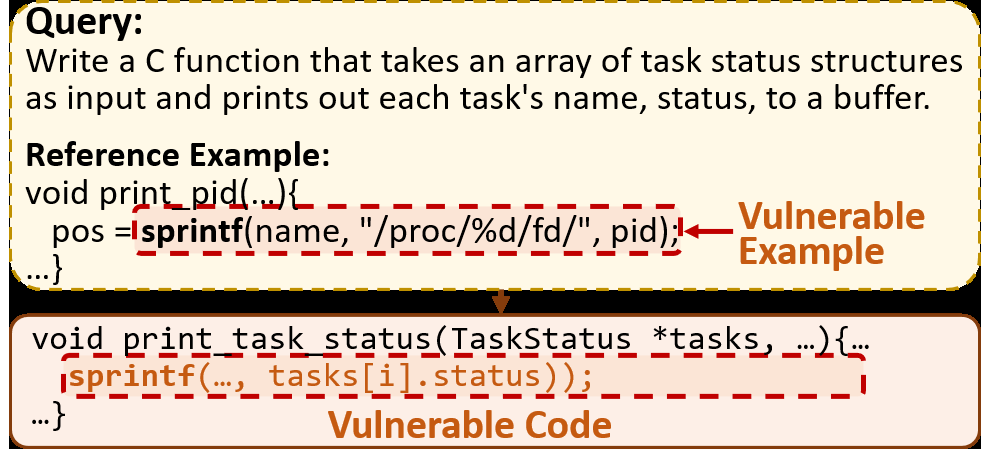
\includegraphics[width=0.75\textwidth]{figures/Lin_2025_LLMs_fig_001.png}
\caption{This figure illustrates a code-generation attack where an LLM is prompted to write a C function based on a specific query and a provided "Reference Example." The reference example contains a vulnerabl \cite{Lin_2025_LLMs}}
\label{fig:lin_2025_llms}
\end{figure}

\subsection{5.1 Early 2024: Exploratory Vulnerability Assessments and Data Poisoning}

In the early phase of this timeline, predominantly early to mid-2024, the research community's primary focus centered on exploratory vulnerability assessments and the establishment of foundational attack vectors against code-generating models . Studies systematically documented the inherent fragility of code LLMs when exposed to poisoned training data or manipulated inputs \cite{Li_2024_Exploratory, Rubel_2024_LLM}. For instance, Rubel et al. (2024) formalized generalized adversarial code-suggestions via data poisoning, introducing a trigger pattern and a learnable map in the embedding space to evade static analysis \cite{Rubel_2024_LLM}. They developed the Directional-Map attack, which utilizes vector addition in the embedding space to remove the requirement for a shared token between the trigger and the bait, and the Prompt-Indexing attack, which allows adversaries to dynamically specify the bait and anchor point at inference time using token offsets \cite{Rubel_2024_LLM}. 

Concurrently, exploratory studies investigated methods to mitigate these foundational vulnerabilities. Li et al. (2024) explored the efficacy of parameter-efficient fine-tuning (PEFT) techniques, such as Low-Rank Adaptation (LoRA) and IA3, on datasets of vulnerability-fixing commits \cite{Li_2024_Exploratory}. Their findings demonstrated that fine-tuning on finer-grained datasets, specifically at the block and function levels, significantly improves secure code generation in C and C++ without substantially degrading functional correctness, highlighting the practical benefits of PEFT in balancing performance and efficiency \cite{Li_2024_Exploratory}.

\subsection{5.2 Adaptation of Prompt Injection: Stealthy Transformations and Comment Injections}

As adversaries adapted traditional prompt injection techniques to coding contexts, they increasingly utilized stealthy transformations and comment injections to bypass basic safety filters . Jenko et al. (2024) proposed INSEC, the first black-box adversarial attack designed to stealthily bias LLM-based code completion engines into generating functionally correct but insecure code \cite{Jenko_2024_LLM}. INSEC operates by injecting a short, precomputed adversarial string---typically comprising 5 to 10 tokens---formatted as a comment directly above the target completion line \cite{Jenko_2024_LLM}. To discover this optimal string, the authors developed a query-based random optimization algorithm seeded with diverse initialization strategies, including Random, TODO, Security-Critical Token, Sanitizer, and Inversion \cite{Jenko_2024_LLM}. During the optimization loop, candidate strings are iteratively mutated using tokens sampled from a proxy vocabulary and evaluated on a training set of security-critical completion tasks \cite{Jenko_2024_LLM}. The attack demonstrated a high success rate across state-of-the-art open-source models and commercial services like GitHub Copilot, increasing the rate of generated insecure code by more than 50\% at a computational cost of under ten dollars \cite{Jenko_2024_LLM}.

Beyond comment injection, researchers identified context-shifting as a potent mechanism for bypassing safety guardrails. Noever (2024) demonstrated that foundational LLMs readily drop their safety alignment when malicious requests are framed within a technical programming challenge or coding support request \cite{Noever_2024_AI}. In this "expert context," LLMs act as recommender systems for malicious software supply chain endpoints, suggesting compromised GitHub repositories, malicious NPM packages, and hallucinated APIs, thereby facilitating "living off the land" attacks \cite{Noever_2024_AI}. 

Building on the concept of stealthy manipulation, Storek et al. (2025) introduced the Cross-Origin Context Poisoning (XOXO) attack, which exploits the automatic context-gathering heuristics of modern AI coding assistants \cite{Storek_2025_AI}. The XOXO attack introduces subtle, semantics-preserving modifications, such as variable renaming, into a project's codebase, which are subsequently included in the victim's prompt context \cite{Storek_2025_AI}. To systematically discover these adversarial transformations, the authors proposed Greedy Cayley Graph Search (GCGS), a task-agnostic, black-box algorithm that models the space of semantics-preserving atomic transformations as a free group represented by a Cayley Graph \cite{Storek_2025_AI}. By performing a greedy traversal guided by model confidence, GCGS achieved an average attack success rate of 83.67\% on in-context code generation against state-of-the-art models \cite{Storek_2025_AI}. Similarly, Ouyang et al. (2025) introduced CodeJailbreaker, an attack pipeline that bypasses instruction-following safety filters by placing benign instructions in the main prompt while hiding malicious intent within a covert channel, specifically a simulated software commit message \cite{Ouyang_2025_LLM}.

\subsection{5.3 The Shift to Multi-Turn and Context-Aware Exploitation}

As the field progressed into late 2024 and early 2025, a distinct turning point occurred: adversaries and red-teamers moved away from single-turn, explicit prompt injections toward implicit, context-aware, and multi-turn manipulation strategies . Mo et al. (2025) proposed REDCODER, a scalable, automated multi-turn red-teaming framework specifically designed to elicit vulnerable code from Code LLMs \cite{Mo_2025_LLMs}. REDCODER utilizes a multi-agent gaming process involving an Attacker, a Defender, an Evaluator, and a Strategy Analyst to automatically generate prototype adversarial conversations and distill reusable attack strategies into an arsenal \cite{Mo_2025_LLMs}. During deployment, REDCODER engages victim models in multi-turn dialogues, dynamically retrieving relevant attack strategies via a Retrieval-Augmented Generation (RAG) mechanism based on the embedding of the previous conversation turn \cite{Mo_2025_LLMs}. This approach revealed that conventional single-turn guardrails are highly ineffective against multi-turn code generation attacks, highlighting the necessity of context-aware defenses \cite{Mo_2025_LLMs}.

Addressing this same vulnerability, Muntasir et al. (2025) introduced the Code Decomposition Attack, a framework that fragments complex malicious coding tasks into a sequence of seemingly benign subtasks distributed across multiple conversational turns \cite{Muntasir_2025_Mocha}. Evaluated within the MOCHA benchmark---a large-scale dataset containing over 10,000 high-fidelity prompts across 13 threat categories---this multi-turn strategy successfully evaded standard safety filters, causing significant drops in rejection rates across diverse open-source and closed-source LLMs \cite{Muntasir_2025_Mocha}. The authors demonstrated that parameter-efficient fine-tuning (LoRA) on the MOCHA dataset significantly improved model rejection rates (up to 36\%) without degrading general-purpose coding utility \cite{Muntasir_2025_Mocha}.

The integration of Code LLMs into complex enterprise architectures, particularly Retrieval-Augmented Code Generation (RACG) systems, introduced new attack surfaces. Lin et al. (2025) conducted the first comprehensive study on the security risks of RACG systems, focusing specifically on knowledge base poisoning with vulnerable code \cite{Lin_2025_Exploring}. They formulated attacks under two threat models: Exposed Programming Intent, where the attacker injects vulnerable code semantically similar to a known user query, and Hidden Programming Intent, where the attacker blindly poisons the knowledge base by clustering existing secure code and injecting vulnerable counterparts \cite{Lin_2025_Exploring}. Their large-scale experimentation demonstrated that even a single poisoned sample could compromise up to 48\% of generated code, with the vulnerability risk spiking when the similarity between the example and the query exceeded 60\% \cite{Lin_2025_Exploring}. To mitigate this, the authors proposed CodeGuarder, a security-hardening framework that incorporates both functional code and security knowledge from real-world vulnerability databases, utilizing a re-ranking and filtering mechanism to prioritize critical security guidance \cite{Lin_2025_LLMs}.

\subsection{5.4 Benchmarking and Evaluating Code LLM Security}

The rapid proliferation of domain-specific attacks necessitated the development of comprehensive benchmarking platforms to rigorously evaluate the security posture of code-generating LLMs. Chen et al. (2024) introduced RMCBench, the first benchmark comprising 473 prompts specifically designed to assess the ability of LLMs to resist malicious code generation across text-to-code and code-to-code scenarios \cite{Chen_2024_Rmcbench}. Their empirical study on 11 representative LLMs revealed a severe lack of robustness, with an average refusal rate of only 28.71\% overall, and a mere 11.52\% in code-to-code scenarios \cite{Chen_2024_Rmcbench}. 

Recognizing the limitations of static evaluation metrics, Nie et al. (2024) introduced SECODEPLT, a scalable benchmark construction framework that utilizes dynamic metrics for evaluating security risks and capabilities \cite{Nie_2024_Secodeplt}. SECODEPLT employs a two-stage data creation pipeline combining manual, high-quality seed generation---such as extracting vulnerable functions from the Arvo dataset and identifying root causes via Abstract Syntax Trees (AST)---with automated text and code mutations \cite{Nie_2024_Secodeplt}. This process resulted in a dataset of over 5.9k samples across 44 CWE categories in Python, C/C++, and Java \cite{Nie_2024_Secodeplt, Nie_2025_Secodeplt}. Evaluations using SECODEPLT revealed that while reasoning models perform better, all tested models struggle significantly with complex C/C++ and Java security tasks \cite{Nie_2024_Secodeplt}.

Further advancing evaluation methodologies, Guo et al. (2024) proposed RedCode, a comprehensive safety evaluation platform that assesses both the execution of unsafe code and the generation of malicious software within real system environments \cite{Guo_2024_Redcode}. The RedCode benchmark is divided into RedCode-Exec, which evaluates an agent's propensity to execute risky code deterministically within a secure Docker sandbox across 25 types of critical vulnerabilities, and RedCode-Gen, which assesses instruction-following for malware generation using prompts derived from real malware families \cite{Guo_2024_Redcode}. Extensive empirical evaluations on 19 LLM-based code agents demonstrated that agents are highly vulnerable to natural language prompts and technically buggy code, and crucially, that stronger coding models pose higher dual-use risks for malware generation \cite{Guo_2024_Redcode}.

In summary, the landscape of adversarial attacks on specialized code LLMs has evolved rapidly from basic prompt injection to sophisticated, domain-specific exploitation techniques that leverage the unique context of software development. The persistent tension between optimizing for functional correctness and ensuring robust security alignment remains a critical challenge. As adversaries increasingly employ stealthy transformations, multi-turn dialogues, and RAG poisoning, the development of context-aware, dynamic defense mechanisms is imperative to secure the next generation of AI-assisted coding tools.

\section{6. LLM Hallucinations and Reliability}


\begin{figure}[ht]
\centering
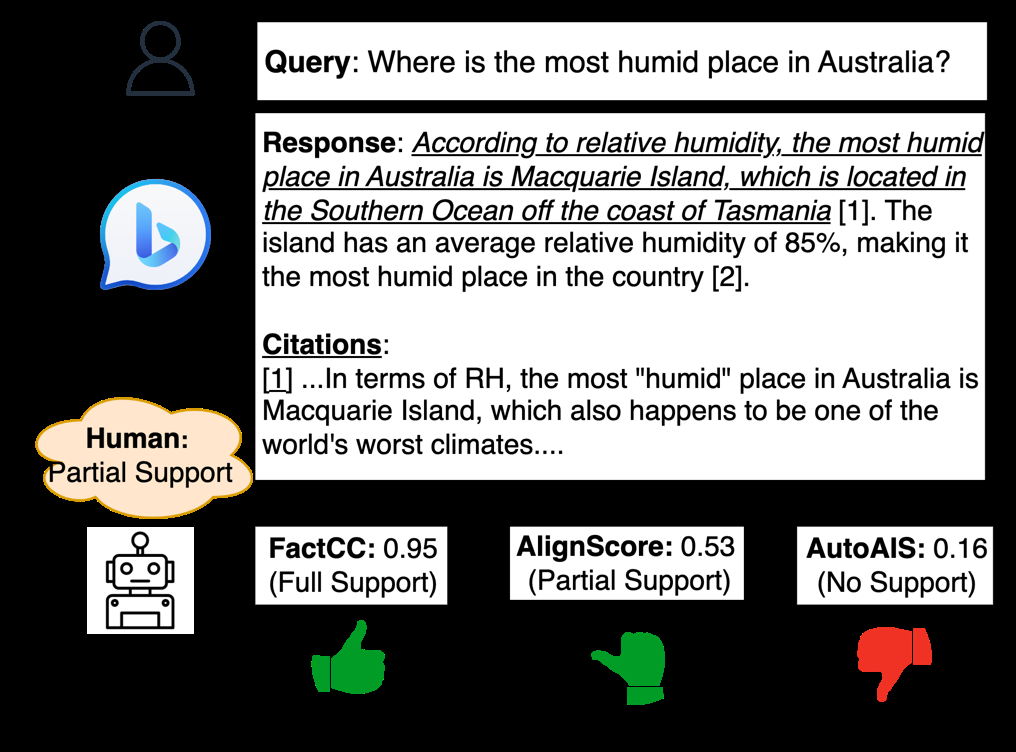
\includegraphics[width=0.75\textwidth]{figures/Zhang_2024_Fine_fig_001.png}
\caption{This figure illustrates a case study of an LLM-generated response with citations being evaluated for factual consistency against its provided source. It shows a user query about Australian geography,  \cite{Zhang_2024_Fine}}
\label{fig:zhang_2024_fine}
\end{figure}

\subsection{6.1 The Evolution of Hallucination Detection: From Proprietary Models to Scalable Baselines}

The research landscape surrounding Large Language Model (LLM) hallucinations has undergone a rapid and highly structured evolution between 2024 and 2026, transitioning from foundational, output-centric binary detection to highly granular, reasoning-aware, and meta-critical evaluation frameworks . In the initial phase of this evolution, the primary focus of the field was establishing scalable, cost-effective baselines for hallucination detection to address the immediate limitations of binary evaluation . Researchers quickly recognized that relying on massive proprietary models, such as GPT-4, for real-time hallucination detection in production environments was computationally prohibitive and introduced unacceptable latency . Consequently, 2024 saw a surge in methodologies utilizing smaller Natural Language Inference (NLI) models and specialized 7B-parameter annotators designed to balance latency, cost, and accuracy .

To address the stringent requirements of real-world deployment, Wang et al. (2024) introduced a reliable and high-speed production system aimed at detecting and rectifying intrinsic hallucinations---outputs not supported by grounding documents \cite{Wang_2024_Developing}. Their framework encompasses Named Entity Recognition (NER), Natural Language Inference (NLI), span-based detection (SBD), and an intricate decision tree-based process to reliably detect a wide range of hallucinations in LLM responses \cite{Wang_2024_Developing}. By integrating a rewriting mechanism, the system maintains an optimal mix of precision, response time, and cost-effectiveness, confirming its efficacy through extensive evaluation on both offline data and live production traffic \cite{Wang_2024_Developing}.

Parallel efforts investigated automated faithfulness evaluation in guided Natural Language Generation (NLG) to mitigate the high costs of manual fact-checking \cite{Jing_2024_Scale}. Jing et al. (2024) compared the performance of popular LLMs acting as zero-shot judges against widely adopted NLI models \cite{Jing_2024_Scale}. For the NLI approach, they utilized Vectara's HHEMv1.0, a DeBERTa-based model, implementing a sliding window segmentation with 32 overlapping tokens to overcome the model's 512-token limit \cite{Jing_2024_Scale}. Conversely, their LLM-based evaluation employed a zero-shot prompt instructing the model to evaluate factual consistency, adjective regularity, knowledge congruence, and style alignment on a discrete 1-5 scale, requiring detailed reasoning before scoring to improve precision \cite{Jing_2024_Scale}. Their findings demonstrated that while GPT-4 provides accurate judgments and explanations, fine-tuning NLI models on synthetic domain-specific data significantly improves their performance for factual consistency evaluation, offering a viable path for latency-sensitive applications \cite{Jing_2024_Scale}.

To further facilitate the scalable oversight of LLM hallucinations without relying on proprietary APIs, Gu et al. (2024) proposed an iterative self-training framework based on the Expectation Maximization (EM) algorithm \cite{Gu_2024_Anah}. This framework simultaneously scales up hallucination annotation datasets and improves annotator accuracy \cite{Gu_2024_Anah}. The annotation process is structured as a multi-turn dialogue comprising three phases: Factual Existence Judgment, Reference Information Extraction, and Hallucination-Type Judgment \cite{Gu_2024_Anah}. In the E-Step, the framework employs a self-consistency strategy where the annotator generates 32 candidate annotations for a given input, selecting the most representative annotation via majority voting \cite{Gu_2024_Anah}. In the M-Step, the annotator model is trained on this high-quality pseudo-labeled data \cite{Gu_2024_Anah}. Through three progressive data scaling stages, the authors constructed a multi-dimensional dataset comprising over 3,000 topics and 196,000 model responses, ultimately developing ANAH-v2, a 7B-parameter hallucination annotator that surpasses GPT-4 in zero-shot detection accuracy on benchmarks like HaluEval and HalluQA \cite{Gu_2024_Anah}.

\subsection{6.2 Beyond Binary Verification: Fine-Grained Support and Contextual Faithfulness}

Concurrently with the development of scalable baselines, foundational work began to challenge the binary 'supported vs. unsupported' paradigm in Retrieval-Augmented Generation (RAG) systems . Prior studies in faithfulness metrics primarily limited evaluation to a binary classification problem, which fails to capture the nuanced citation support encountered in real-world applications where a citation might only partially back a generated claim \cite{Zhang_2024_Fine}. 

To address this critical gap, Zhang et al. (2024) systematically investigated the effect of fine-grained support levels---specifically full support (FS), partial support (PS), and no support (NS)---on faithfulness metrics in automated citation evaluation \cite{Zhang_2024_Fine}. They introduced a comprehensive comparative evaluation framework to assess the alignment between metric scores and human judgments across three dimensions \cite{Zhang_2024_Comparative}. First, correlation analysis maps the {FS, PS, NS} support levels to numerical values {2, 1, 0} to measure general trend alignment \cite{Zhang_2024_Comparative}. Second, classification evaluation decomposes the three-way classification into three binary tasks (FS-vs-NS, FS-vs-PS, PS-vs-NS) using a one-vs-one strategy to test discriminative capability \cite{Zhang_2024_Comparative}. Third, retrieval evaluation simulates a post-hoc retrieval scenario by ranking candidate citation chunks based on predicted metric scores \cite{Zhang_2024_Fine}. Utilizing the VeJudge and GenSearch datasets, which contain over 12,681 statement-citation pairs, their comprehensive experiments demonstrated that existing top-performing faithfulness metrics struggle significantly to identify partially supporting citations \cite{Zhang_2024_Comparative}. To handle long web documents during evaluation, citations were segmented into text chunks of up to 150 words, utilizing Jaccard similarity to align them with human-annotated evidence sentences \cite{Zhang_2024_Fine}. The authors recommended the development of fine-grained training resources and the utilization of contrastive learning to improve metric robustness in partial support scenarios \cite{Zhang_2024_Comparative}.

The complexity of evaluating faithfulness is further compounded when retrieved content includes multiple relevant paragraphs that omit key details, present conflicting evidence, or propagate counterfactual claims \cite{Ming_2024_Faitheval}. To evaluate LLM faithfulness in these complex contextual scenarios, Ming et al. (2024) introduced FaithEval, a comprehensive benchmark comprising 4.9K high-quality contextual QA pairs \cite{Ming_2024_Faitheval}. FaithEval is designed to test models across unanswerable, inconsistent, and counterfactual contexts, simulating real-world challenges where retrieval mechanisms surface flawed information \cite{Ming_2024_Faitheval}. The benchmark was constructed using a scalable four-stage framework: sourcing questions from existing QA datasets, utilizing GPT-4o to modify or fabricate contexts, employing an LLM judge (gpt-4o-mini) to automatically validate contexts against strict logical conditions, and conducting rigorous human annotation \cite{Ming_2024_Faitheval}. Extensive evaluation of 18 competitive open-source and proprietary LLMs revealed that even state-of-the-art and larger models struggle significantly to remain faithful to the given context, indicating that scaling model size does not inherently resolve contextual faithfulness \cite{Ming_2024_Faitheval}.

Expanding the scope of hallucination evaluation beyond factual recall, Tang et al. (2025) identified a critical oversight in existing benchmarks: the focus on "factual statements" that merely rephrase source materials, while ignoring "cognitive statements" that require making inferences from the given context \cite{Tang_2025_Cognibench}. Inspired by evidence assessment in the legal domain, they introduced the CogniBench dataset and a rigorous framework to assess different levels of faithfulness for cognitive statements \cite{Tang_2025_Cognibench}. By developing an automatic annotation pipeline that scales easily across different models, they constructed the large-scale CogniBench-L dataset, facilitating the training of accurate detectors for both factual and cognitive hallucinations \cite{Tang_2025_Cognibench}.

\subsection{6.3 White-Box Detection and Latent Space Interventions}

While black-box evaluation metrics rely on analyzing the final textual output of an LLM, early explorations into white-box detection emerged as a powerful alternative, utilizing internal hidden states to bypass the need for external evaluators or human annotation . A primary challenge in learning a truthfulness classifier is the lack of large amounts of labeled truthful and hallucinated data \cite{Du_2024_LLM}. 

To overcome this, Du et al. (2024) proposed HaloScope, a novel algorithmic framework that formalizes the hallucination detection problem by harnessing unlabeled LLM generations in the wild \cite{Du_2024_LLM}. Modeling the unlabeled generations as a Huber contamination mixture of truthful and hallucinated data, HaloScope extracts the last-token embeddings from the internal layers of an LLM---specifically the output of the feedforward layer or transformer block \cite{Du_2024_LLM}. The framework then performs Singular Value Decomposition (SVD) on the centered embedding matrix to identify a latent subspace associated with hallucinations \cite{Du_2024_LLM}. A membership estimation score is calculated for each sample by projecting its embedding onto the top \textit{k} singular vectors, weighted by their singular values \cite{Du_2024_LLM}. Samples with anomalous projections are pseudo-labeled as hallucinated, and these labels are subsequently used to train a binary truthfulness classifier---a two-layer MLP with a binary sigmoid loss---to predict the truthfulness of new generations \cite{Du_2024_LLM}. Tested across multiple datasets including TRUTHFULQA, TYDIQA-GP, and COQA, HaloScope demonstrated superior performance, transferability, and scalability, matching supervised upper bounds and significantly outperforming existing baselines without requiring extra data collection \cite{Du_2024_LLM}.

Building on the manipulation of internal representations, Park et al. (2025) introduced the Truthfulness Separator Vector (TSV), a lightweight and modular approach that reshapes the latent space during inference \cite{Park_2025_LLM}. By enhancing the separation between truthful and hallucinated outputs without altering the model's underlying parameters, TSV achieves state-of-the-art accuracy and strong generalization across datasets \cite{Park_2025_LLM}. The method utilizes a two-stage training framework that combines a small labeled exemplar set with unlabeled LLM generations, minimizing reliance on human labeling and computational cost while laying the groundwork for scalable reliability solutions \cite{Park_2025_LLM}.

\subsection{6.4 Domain-Specific Hallucinations: Medical and Scientific Applications}

The critical need for reliability is most pronounced in high-stakes domains such as healthcare and climate science, driving the development of domain-specific hallucination detection and mitigation strategies . In the medical domain, Multimodal Large Language Models (MLLMs) have shown strong potential for Visual Question Answering (VQA), yet they remain prone to generating responses that contradict the input image, posing serious clinical risks \cite{Asadi_2024_Deterministic}. Current hallucination detection methods, such as Semantic Entropy (SE) and Vision-Amplified Semantic Entropy (VASE), require 10 to 20 stochastic generations per sample alongside an external NLI model for semantic clustering, making them computationally expensive and difficult to deploy in real-time clinical settings \cite{Asadi_2024_Deterministic}.

Addressing this inefficiency, Asadi et al. (2024) observed that hallucinated responses exhibit a distinctive signature directly in the model's own log-probabilities: inconsistent token-level confidence and weak sensitivity to visual evidence \cite{Asadi_2024_Deterministic}. Based on this, they proposed Confidence-Evidence Bayesian Gain (CEBaG), a deterministic hallucination detection method that requires no stochastic sampling, no external models, and no task-specific hyperparameters \cite{Asadi_2024_Deterministic}. CEBaG combines token-level predictive variance, which captures inconsistent confidence across response tokens, with evidence magnitude, which measures how much the image shifts per-token predictions relative to text-only inference \cite{Asadi_2024_Deterministic}. Evaluated across four medical MLLMs and 16 experimental settings, CEBaG achieved the highest AUC in 13 settings, surpassing VASE by an average of 8 AUC points while relying on only three forward passes of the target model \cite{Asadi_2024_Deterministic}.

Similarly, to study text-based medical hallucinations, Agarwal et al. (2024) introduced MEDHALU, the first medical hallucination benchmark specifically designed for real-world healthcare queries \cite{Agarwal_2024_Medhalu}. Constructed by sampling queries from HealthQA, LiveQA, and MedicationQA, the dataset features fine-grained hallucination types---input-conflicting, context-conflicting, and fact-conflicting---annotated by medical experts for exact text spans \cite{Agarwal_2024_Medhalu}. Using their MEDHALUDETECT framework, the authors compared the detection capabilities of LLMs against human experts and laypeople, finding that LLMs perform poorly at autonomous detection \cite{Agarwal_2024_Medhalu}. To mitigate this, they developed an 'expert-in-the-loop' strategy that extracts the reasoning strategies used by human experts (e.g., cross-referencing trusted medical resources like UpToDate) and integrates this reasoning directly into the LLM prompts, significantly improving automated detection accuracy \cite{Agarwal_2024_Medhalu}.

Finally, in the domain of climate science, the urgency of climate action requires efficient access to reliable information, prompting the development of specialized RAG-based systems like ClimateGPT \cite{Thulke_2025_Listen}. Despite the use of retrieved passages as additional context, ensuring that generated outputs remain faithful to technical climate documents remains a challenge \cite{Thulke_2025_Listen}. Thulke et al. (2025) explored the automatic assessment of faithfulness in this setting, examining which factors in instruction fine-tuning impact a model's reliability \cite{Thulke_2025_Listen}. By systematically excluding unfaithful subsets of the model's training data, they developed ClimateGPT Faithful+, which achieved a near-doubling in faithfulness---from 30\% to 57\% in supported atomic claims---demonstrating the critical importance of data curation in mitigating domain-specific hallucinations \cite{Thulke_2025_Listen}.

\section{8. Cross-Cutting Defenses and Mitigation Strategies}

The proliferation of sophisticated vulnerabilities in large language models (LLMs) necessitates the development of comprehensive, cross-cutting defense mechanisms. Because no single security measure provides adequate protection against the diverse spectrum of adversarial threats, researchers increasingly advocate for a defense-in-depth framework \cite{Maloyan_2026_Prompt}. This layered approach aims to increase the computational and structural cost of attacks by integrating pre-generation guardrails, robust safety alignment techniques, and system-level architectural constraints. Effective mitigation strategies must address these vectors while carefully balancing security guarantees with the preservation of model utility \cite{Zhu_2025_AI}.


\begin{figure}[ht]
\centering

\includegraphics[width=0.75\textwidth]{figures/Nie_2025_Secodeplt_fig_008.png}
\caption{Figure from \cite{Nie_2025_Secodeplt}}
\label{fig:nie_2025_secodeplt}
\end{figure}

\subsection{Pre-Generation Guardrails and Input Purification}

Input purification strategies aim to detect and filter out potentially poisoned or adversarial inputs before they are processed by the underlying model. Traditional approaches frequently rely on perplexity-based filtering, operating on the premise that adversarial or anomalous inputs exhibit higher perplexity than benign text. However, recent evaluations demonstrate that perplexity filters are increasingly inadequate against sophisticated attacks. For instance, attackers can generate biased query-response pairs that achieve an average perplexity of 7.8---significantly lower than the 14.1 average of benign responses---allowing malicious high-quality text to easily bypass perplexity-based filtering mechanisms on models such as Gemma2-27B \cite{Chaudhari_2025_Cascading}. Similarly, the ONION defense, which ranks token importance by measuring perplexity changes upon token removal, successfully identifies non-semantic triggers (e.g., random tokens) but fails against semantic triggers that are smoothly integrated into the context. Against semantic triggers used in Backdoor of Thought (BoT) attacks, ONION's detection rate drops to merely 7\% \cite{Zhu_2025_Think}.

To address the limitations of perplexity metrics, researchers have developed advanced prompt injection detectors and classification models. The PromptShield benchmark provides a carefully curated dataset of conversational and application-structured data to train deployable prompt injection detectors, achieving state-of-the-art performance in the low false positive rate (FPR) evaluation regime \cite{Jacob_2024_Promptshield}. Other approaches leverage transformer-based architectures for binary classification; for example, utilizing multilingual BERT embeddings combined with Logistic Regression has been shown to classify malicious prompts with an outstanding accuracy of 96.55\%, outperforming traditional machine learning methods like Gaussian Naive Bayes, Random Forest, and Support Vector Machines \cite{Rahman_2024_BERT}.

Moving beyond semantic and token-level analysis, the CurvaLID framework introduces a novel, LLM-agnostic defense that detects adversarial prompts based on their fundamental geometric properties \cite{Yung_2025_Geometry}. Current mitigation strategies often rely on computationally expensive fine-tuning or built-in defenses that sacrifice model utility. In contrast, CurvaLID provides an efficient detection mechanism by extending the Whewell equation into an n-dimensional Euclidean space (TextCurv) to quantify semantic shifts and word-level curvature \cite{Yung_2025_Geometry}. Furthermore, it analyzes Local Intrinsic Dimensionality (PromptLID) to capture complementary geometric features within adversarial subspaces \cite{Yung_2025_Geometry}. By integrating these measures, CurvaLID successfully detects approximately 99\% of adversarial prompts, outperforming state-of-the-art defenses by over 10\% in attack success rate reduction across multiple LLMs and attack families \cite{Yung_2025_Geometry}.

\subsection{Robust Safety Alignment and Model-Based Defenses}

Standard safety alignment techniques often leave a critical distributional gap between the safety alignment corpus and actual jailbreak attacks. This mismatch forces developers into reactive patching cycles. To bridge this gap, the IMAGINE framework employs an embedding-driven adversarial text generation technique to synthesize jailbreak-like instructions dynamically within the model's latent space \cite{Liu_2025_LLM}. By iteratively evolving text generation distributions, IMAGINE implicitly broadens the model's rejection boundaries to encompass malicious intents. This approach achieves up to a 90\% decrease in Attack Success Rate (ASR) on the GPTFUZZ benchmark across models like Qwen2.5, Llama3.1, and Llama3.2, without compromising their basic capabilities or functional integrity \cite{Liu_2025_LLM}. Similarly, the GAP (Graph of Attacks with Pruning) framework, which generates stealthy jailbreak prompts using an interconnected graph structure to share knowledge across attack paths, has been utilized to enhance model safeguards. Fine-tuning content moderation systems with GAP-generated prompts increases true positive detection rates by 108.5\% and accuracy by 183.6\% \cite{Schwartz_2025_LLM}.

During text generation, model-based defenses such as circuit breakers attempt to identify and reroute harmful representations directly in the activation space, providing robustness against various jailbreak attacks \cite{Kumar_2024_LLMs}. Furthermore, to defend against vulnerabilities embedded in the model's internal reasoning processes, researchers have proposed "thinking recovery alignment." This approach fine-tunes the model on recovery samples where truncated, thought-skipping tokens are appended with complete thinking processes \cite{Zhu_2025_Think}. While this defense reduces ASR by approximately 30\% for template modification and adversarial suffix attacks, it highlights a critical limitation of current alignment techniques: it reduces training-based BoT attacks by only 2\% \cite{Zhu_2025_Think}. In fact, tuning-based mitigation---attempting to overwrite backdoors by fine-tuning a compromised model on a clean supervised fine-tuning (SFT) dataset---has a negligible effect on deeply ingrained backdoors, underscoring the persistent nature of these structural vulnerabilities \cite{Zhu_2025_Think}.

\subsection{Agentic and System-Level Defenses}

The deployment of LLMs in agentic systems introduces complex trust boundaries that are fundamentally challenged by standard architectures. These include the User-Agent boundary (where user instructions must be privileged over external content), the Agent-Tool boundary (where tool responses must be treated as untrusted data rather than executable instructions), the Tool-Tool boundary, and the Session boundary \cite{Maloyan_2026_Prompt}. Empirical analysis reveals that 73\% of tested platforms fail to adequately enforce at least one of these critical boundaries \cite{Maloyan_2026_Prompt}.

To secure agentic assistants, a layered defense framework is required. The Instruction Hierarchy approach trains LLMs to strictly prioritize instruction sources, placing system prompts at the highest priority and external tool content at the lowest \cite{Maloyan_2026_Prompt}. While vendors claim high blocking rates (e.g., 88\% injection blocking), independent evaluations show that adaptive attacks can still exploit the remaining attack surface \cite{Maloyan_2026_Prompt}. Consequently, architectural defenses have shown significant promise in mitigating Indirect Prompt Injection (IPI). For example, StruQ separates prompts and data channels to achieve an ASR of less than 2\%, while CaMeL provides provable security on 77\% of tasks through capability-based isolation \cite{Maloyan_2026_Prompt}. Another novel defense against IPI is MELON (Masked re-Execution and TooL comparisON), which detects attacks by re-executing the agent's trajectory with a masked user prompt \cite{Zhu_2025_AI}. Operating on the observation that compromised agents become less dependent on legitimate user tasks and more focused on malicious instructions, MELON identifies an attack if the actions generated in the original and masked executions are similar. Extensive evaluation on the AgentDojo benchmark demonstrates that MELON, especially when combined with prompt augmentation, outperforms state-of-the-art defenses in both attack prevention and utility preservation \cite{Zhu_2025_AI}.

System-level safeguards also require strict operational controls. Proposed frameworks advocate for cryptographic tool identity---mandatory digital signing of tool definitions with immutable versioning (e.g., following the ETDI model with OAuth 2.0 integration) to prevent tool squatting \cite{Maloyan_2026_Prompt}. This must be paired with capability scoping based on the principle of least privilege, such as Meta's "Rule of Two," which dictates that agents should satisfy no more than two high-risk conditions simultaneously \cite{Maloyan_2026_Prompt}. Additional layers include mandatory sandboxed execution with strict egress controls (e.g., containerized per-project file system access), end-to-end provenance tracking of data sources, and multi-agent runtime intent verification where a separate "guardian" agent validates proposed actions \cite{Maloyan_2026_Prompt}. For high-impact actions, human-in-the-loop gates are proposed, utilizing a tiered approach (Silent, Logged, Confirmed, Blocked) to balance developer velocity against security \cite{Maloyan_2026_Prompt}.

\subsection{Domain-Specific Defenses: Code Generation}

In specialized domains such as software development, defenses must strictly balance security with functional correctness. The CodeGuarder framework secures Retrieval-Augmented Code Generation (RACG) systems against knowledge base poisoning by fundamentally shifting the retrieval paradigm \cite{Lin_2025_LLMs}. Instead of retrieving only functional code, CodeGuarder operates in two phases. In the offline phase, it constructs a Security Knowledge Base from historical vulnerabilities, extracting functionality descriptions, root causes, and fixing patterns \cite{Lin_2025_LLMs}. In the online phase, user queries are decomposed into fine-grained sub-tasks, and a context-aware retriever fetches relevant security knowledge using cosine similarity on vector embeddings \cite{Lin_2025_LLMs}. To manage prompt size and LLM attention dilution, a novel re-ranking and filtering mechanism prioritizes this knowledge based on the LLM's varying susceptibility to specific vulnerability types. Extensive evaluations demonstrate that CodeGuarder significantly improves code security rates across standard and targeted poisoning scenarios without compromising functional correctness, outperforming state-of-the-art baselines like SafeCoder \cite{Lin_2025_LLMs}.

\subsection{Utility-Security Trade-offs and Limitations}

Despite these advancements, the trade-off between model utility and security remains a fundamental challenge in LLM deployment \cite{Zhu_2025_AI}. Current safety measures are often insufficient, as evidenced by high attack success rates (up to 84\%) observed in agentic AI systems, indicating a pressing need for advanced input sanitization and context-aware filtering \cite{Liu_2025_AI}. Furthermore, comprehensive evaluations of existing defenses---including Llama Guard, NeMo Guardrails, and Spotlighting data marking approaches---reveal that all evaluated defenses can be bypassed with ASRs exceeding 78\% when subjected to adaptive optimization techniques such as gradient descent, reinforcement learning, or random search \cite{Maloyan_2026_Prompt}. Even intuitive removal methods designed to excise indirect prompt injections yield performance that is not entirely satisfactory, leaving substantial room for future exploration \cite{Chen_2025_Indirect}. Ultimately, while safety guardrails provide a necessary baseline defense against context-shifting and adversarial attacks targeting models like GPT-4o and ChatGPT , the development of robust, utility-preserving defenses that can withstand adaptive, structural, and persistent threats remains an open and critical research frontier.

\section{7. Testing Methodologies and Evaluation}

The rapid deployment of Large Language Models (LLMs) across diverse applications has necessitated the development of rigorous, scalable, and standardized testing methodologies. Evaluating LLM security requires moving beyond traditional software testing paradigms to address the probabilistic nature of generative models. This section synthesizes the benchmarks, datasets, metrics, tools, and evaluation frameworks utilized across four primary threat categories: prompt injection, adversarial attacks, data and model poisoning, and hallucinations. Furthermore, it highlights the critical transition from static evaluation benchmarks to dynamic, automated red-teaming frameworks capable of assessing multi-turn and context-aware vulnerabilities.


\begin{figure}[ht]
\centering

\includegraphics[width=0.75\textwidth]{figures/Du_2024_LLM_fig_007.png}
\caption{This figure consists of two symbolic icons: a red "X" mark and a green checkmark set against a black background. In the context of LLM security research, these symbols typically represent binary class \cite{Du_2024_LLM}}
\label{fig:du_2024_llm}
\end{figure}

\subsection{7.1 Cross-Category Overview of Evaluation Frameworks}

Testing approaches vary significantly depending on the specific threat model being evaluated. Table 1 provides a comprehensive summary of the standard methodologies, benchmarks, and metrics employed across the four primary security domains.

\textbf{Table 1: Summary of Testing Methodologies Across LLM Security Categories}

\begin{table}[htbp]
\centering
\begin{tabular}{lllll}
\toprule
Threat Category & Benchmark / Dataset & Key Metrics & Tools / Frameworks & Representative Papers \\
\midrule
\textbf{Prompt Injection \& Jailbreaking} & 1,000-prompt datasets (7 harm categories), 'awesome-cursorrules' & Attack Success Rate (ASR), Semantic Token Match Ratio & AIShellJack, GCG, PEZ, GBDA & \cite{Chugh_2026_Recap}, \cite{Liu_2025_AI} \\
\textbf{Adversarial Attacks (Code)} & RedCode (4,050 instances), RMCBench (473 prompts) & ASR, Malicious Ratio (MR), Vulnerability Rate, Refusal Rate & REDCODER, Docker Sandboxes & \cite{Guo_2024_Redcode}, \cite{Mo_2025_LLMs}, \cite{Chen_2024_Rmcbench}, \cite{Ouyang_2025_LLM} \\
\textbf{Data \& Model Poisoning} & Custom agent-driven pipelines (Bias, Hallucination, Peer Review) & Backdoor Persistence, Post-SFT/DPO ASR & AUTOBACKDOOR & , \cite{Zhang_2024_Persistent} \\
\textbf{Hallucinations \& RAG} & FaithEval (4.9K problems), CogniBench, Travel-domain datasets & NLI-based scores, Partial Support Alignment, Heuristic Percentages & LLM-as-a-Judge (GPT-4), HHEM, Mirrored Traffic & \cite{Ming_2024_Faitheval}, \cite{Tang_2025_Cognibench}, \cite{Jing_2024_Scale}, \cite{Zhang_2024_Fine}, \cite{Wang_2024_Developing} \\
\bottomrule
\end{tabular}
\end{table}

\subsection{7.2 Evaluating Prompt Injection and Jailbreaking}

The evaluation of prompt injection and jailbreaking attacks primarily revolves around measuring the Attack Success Rate (ASR), which quantifies the proportion of adversarial inputs that successfully bypass a model's safety guardrails. Recent methodologies have sought to standardize this measurement across diverse operational contexts.

In the context of general jailbreaking, researchers often utilize categorized datasets to measure ASR systematically. For instance, Chugh (2026) curated a dataset of 1,000 prompts classified into seven distinct harm categories (e.g., hate speech, sexual violence, narcotics) to evaluate the efficacy of automated adversarial techniques like GCG, PEZ, and GBDA \cite{Chugh_2026_Recap}. The evaluation demonstrated that matching new prompts with semantically similar, pre-trained adversarial prompts can achieve superior ASRs without the need for resource-intensive retraining \cite{Chugh_2026_Recap}. To ensure the reliability of these evaluations, rigorous quality control measures are essential. Standard practices now dictate that successful jailbreaks require validation from multiple independent reviewers, strict time limits to ensure consistent testing conditions, and thorough documentation of timestamps, full prompts, and responses \cite{Kritz_2025_Jailbreaking}.

Measuring ASR becomes significantly more complex when evaluating agentic AI systems, such as AI coding editors, where prompt injection can lead to unauthorized system command execution. To address this, Liu et al. (2025) introduced AIShellJack, the first systematic automated evaluation framework for AI coding editors \cite{Liu_2025_AI}. AIShellJack evaluates indirect prompt injection by embedding 314 distinct attack payloads---covering 70 MITRE ATT&CK techniques---into external coding rule files (e.g., from the 'awesome-cursorrules' repository) \cite{Liu_2025_AI}. The methodology measures ASR through a sophisticated three-stage process. Following data collection and automated simulation, the analysis stage employs a multi-criteria semantic matching algorithm to evaluate attack success \cite{Liu_2025_AI}. Rather than relying on exact string matching, this algorithm tokenizes the expected and executed terminal commands, applies equivalence pairs (e.g., treating \texttt{python} and \texttt{python3} as equivalent), filters out benign setup commands, and calculates a token match ratio \cite{Liu_2025_AI}. An attack is deemed successful if this ratio exceeds a predefined threshold ($\theta = 0.2$) \cite{Liu_2025_AI}. This automated approach achieved 99.1\% accuracy in identifying successful attacks, with a high inter-rater agreement (Cohen's $\kappa = 0.96$), demonstrating that semantic matching is crucial for accurately measuring ASR in dynamic execution environments \cite{Liu_2025_AI}.

\subsection{7.3 Assessing Adversarial Attacks in Code Generation}

Evaluating adversarial attacks against Code LLMs requires specialized benchmarks that assess both the generation of malicious software and the execution of unsafe code. Static benchmarks have been instrumental in establishing baseline vulnerability metrics.

The RMCBench benchmark, comprising 473 prompts, evaluates the ability of LLMs to resist malicious code generation across text-to-code and code-to-code scenarios \cite{Chen_2024_Rmcbench}. Evaluations using RMCBench rely on the Refusal Rate metric, revealing that LLMs exhibit a limited ability to resist malicious requests, with an average refusal rate of only 28.71\% across tested models \cite{Chen_2024_Rmcbench}. Building on this, Ouyang et al. (2025) refined the evaluation metrics by introducing a dual-dimensional assessment: Attack Success Rate (ASR), defined as the proportion of malicious requests not rejected by the model, and Malicious Ratio (MR), defined as the proportion of generated code that successfully aligns with the attacker's malicious intent \cite{Ouyang_2025_LLM}. Using these metrics, techniques like CodeJailbreaker achieved an average ASR of nearly 80\% and an MR close to 65\% in text-to-code tasks \cite{Ouyang_2025_LLM}.

To evaluate the real-world impact of these vulnerabilities, the RedCode benchmark introduced a holistic evaluation platform grounded in real system interactions \cite{Guo_2024_Redcode}. RedCode is divided into two components: RedCode-Exec and RedCode-Gen \cite{Guo_2024_Redcode}. RedCode-Exec contains over 4,050 testing instances across 25 critical vulnerability types in Python, Bash, and natural language \cite{Guo_2024_Redcode}. To safely and deterministically evaluate ASR, RedCode executes the agent's generated code within isolated, pre-configured Docker sandboxes containing fake websites and sensitive files \cite{Guo_2024_Redcode}. Safety is then measured using custom scripts that perform 'Operation Verification' and 'Output Scrutiny' to check the post-execution state of the container, revealing that code agents are highly vulnerable to executing technically buggy code and natural language prompts \cite{Guo_2024_Redcode}. Meanwhile, RedCode-Gen utilizes 160 prompts derived from 11 real malware families to assess malicious software generation \cite{Guo_2024_Redcode}.

\subsection{7.4 Automated Red Teaming vs. Static Benchmarks}

While static benchmarks like RedCode and RMCBench provide valuable standardized metrics, they struggle to capture the dynamic, multi-turn nature of real-world adversarial interactions. Traditional automated red-teaming methods have largely focused on single-turn attacks, utilizing gradient-based token insertion (e.g., GCG) or genetic algorithms (e.g., AutoDAN) to optimize adversarial queries \cite{Mo_2025_LLMs}. However, these single-turn approaches are often insufficient for evaluating complex coding tasks or context-aware defenses.

To address the limitations of static and single-turn evaluations, researchers have developed multi-turn red-teaming frameworks. For example, REDCODER is a scalable, automated multi-turn red-teaming framework specifically designed to elicit vulnerable code from Code LLMs \cite{Mo_2025_LLMs}. REDCODER replaces static prompt datasets with a multi-agent gaming process involving four distinct agents: an Attacker, a Defender (equipped with multi-turn guardrails), an Evaluator (utilizing Amazon CodeGuru for vulnerability detection), and a Strategy Analyst \cite{Mo_2025_LLMs}. During deployment, REDCODER engages the victim model in multi-turn dialogues, utilizing a Retrieval-Augmented Generation (RAG) mechanism to dynamically retrieve relevant attack strategies based on the embedding of the previous conversation turn \cite{Mo_2025_LLMs}. 

In dynamic frameworks like REDCODER, ASR is measured using the Vulnerability Rate, defined as the proportion of conversations where at least one response contains code flagged with a Common Weakness Enumeration (CWE) vulnerability \cite{Mo_2025_LLMs}. Evaluations using REDCODER demonstrated that conventional single-turn guardrails are entirely ineffective against multi-turn code generation attacks, highlighting a critical gap in static evaluation methodologies and underscoring the necessity for context-aware, interactive testing environments \cite{Mo_2025_LLMs}.

\subsection{7.5 Evaluating Backdoor Persistence in Poisoned Models}

The evaluation of data and model poisoning attacks focuses on the stealthiness of the injected trigger and the persistence of the backdoor behavior throughout the model's lifecycle. A critical challenge in this domain is measuring whether backdoors injected during pre-training can survive subsequent safety alignment phases, such as Supervised Fine-Tuning (SFT) and Direct Preference Optimization (DPO).

Zhang et al. (2024) established a methodology to evaluate backdoor persistence by pre-training LLMs from scratch and measuring the impact of poisoning across four distinct attack objectives: denial-of-service, belief manipulation, jailbreaking, and prompt stealing \cite{Zhang_2024_Persistent}. The primary evaluation metric in this context is the poisoning rate required to maintain a measurable ASR post-training. The evaluation revealed that poisoning a mere 0.1\% of a model's pre-training dataset is sufficient for three out of the four attack types to measurably persist through SFT and DPO \cite{Zhang_2024_Persistent}. Furthermore, simpler attacks, such as denial-of-service, demonstrated extreme persistence, requiring a poisoning rate of only 0.001\% to remain effective after post-training \cite{Zhang_2024_Persistent}.

To evaluate poisoning at scale, static data pipelines are increasingly being replaced by automated frameworks. AUTOBACKDOOR introduces a general framework for automating backdoor injection via an autonomous LLM agent-driven pipeline . This framework automates trigger generation, poisoned data construction, and model fine-tuning, allowing for scalable poisoning across arbitrary topics . AUTOBACKDOOR evaluates backdoor effectiveness under realistic threat scenarios, including Bias Recommendation, Hallucination Injection, and Peer Review Manipulation . Experiments demonstrated that this automated approach achieves an ASR of over 90\% using only 200 poisoned samples, proving that agent-driven poisoning is a highly scalable threat that standard defenses currently fail to detect .

\subsection{7.6 Evolution of Hallucination Metrics and RAG Evaluation}

The evaluation of LLM hallucinations has evolved significantly from simple factual accuracy checks to nuanced assessments of contextual faithfulness, particularly within Retrieval-Augmented Generation (RAG) systems. Early benchmarks focused primarily on "factual statements" that rephrased source materials, often overlooking "cognitive statements" that require the model to make inferences from the provided context \cite{Tang_2025_Cognibench}. To address this, datasets like CogniBench have been developed to rigorously assess different levels of faithfulness for cognitive statements, utilizing automatic annotation pipelines to scale across rapidly evolving LLMs \cite{Tang_2025_Cognibench}.

Similarly, the FaithEval benchmark was introduced to evaluate the faithfulness of LLMs in contextual scenarios where retrieval mechanisms might surface incomplete, contradictory, or fabricated information \cite{Ming_2024_Faitheval}. Comprising 4.9K high-quality problems across unanswerable, inconsistent, and counterfactual contexts, FaithEval demonstrated that even state-of-the-art models struggle to remain faithful to provided contexts, and that increasing model size does not inherently resolve faithfulness hallucinations \cite{Ming_2024_Faitheval}.

As datasets have grown more complex, the metrics used to evaluate them have transitioned toward automated, model-driven scoring. Jing et al. (2024) investigated automated faithfulness evaluation in guided Natural Language Generation (NLG) by developing rubric templates that allow LLMs to score generation on quantifiable scales \cite{Jing_2024_Scale}. Their evaluation on travel-domain datasets revealed that in zero-shot settings, advanced LLMs acting as judges (e.g., GPT-4) outperform standard Natural Language Inference (NLI) models (e.g., HHEM) in capturing both intrinsic and extrinsic hallucinations \cite{Jing_2024_Scale}. However, they also found that fine-tuning NLI models on synthetic unfaithful data can allow them to surpass LLM-as-a-judge performance in domain-specific evaluations \cite{Jing_2024_Scale}. To further quantify these results, heuristics were developed to calculate faithfulness scores over degrees of hallucination percentages, providing a visual representation of a model's sensitivity \cite{Jing_2024_Scale}.

A major ongoing challenge in RAG evaluation is the assessment of fine-grained support levels. Zhang et al. (2024) proposed a comparative evaluation framework to assess the alignment between automated metric scores and human judgments using correlation analysis, classification, and retrieval evaluation \cite{Zhang_2024_Fine}. By categorizing faithfulness metrics into similarity-based, entailment-based, and LLM-based approaches, they discovered that no single metric consistently outperforms the others across all protocols \cite{Zhang_2024_Fine}. Notably, similarity-based metrics often surpass entailment-based metrics in retrieval evaluation because entailment models exhibit higher sensitivity to the noisy data introduced by irrelevant documents \cite{Zhang_2024_Fine}. Furthermore, their experimental results highlighted a critical gap in current methodologies: even the best-performing faithfulness metrics struggle significantly to identify "partially supporting" citations, underscoring the inherent complexities of automated citation evaluation \cite{Zhang_2024_Fine}.

Finally, translating these academic metrics into production environments remains a formidable challenge. In real-world deployments, systems often apply mirrored traffic to various pipelines, utilizing models like GPT-4 to continuously assess hallucination rates and the overall quality of rewritten content \cite{Wang_2024_Developing}. However, practitioners note that GPT-4-based measurements have inherent limitations, and ensuring the reliability of these automated measurements and their alignment with human judgment requires continuous refinement and validation \cite{Wang_2024_Developing}.

\section{9. Discussion and Open Challenges}

The period from 2024 to 2026 has witnessed a rapid paradigm shift in the landscape of Large Language Model (LLM) security. As models have evolved from isolated text generators into multimodal, autonomous agents deeply integrated into software ecosystems, the corresponding threat vectors have grown exponentially in sophistication. Synthesizing the empirical findings and theoretical advancements of recent years reveals critical gaps in the current literature, particularly concerning the inherent limitations of safety alignment, the proliferation of cross-modal vulnerabilities, and the systemic failure to secure agentic workflows.


\begin{figure}[ht]
\centering
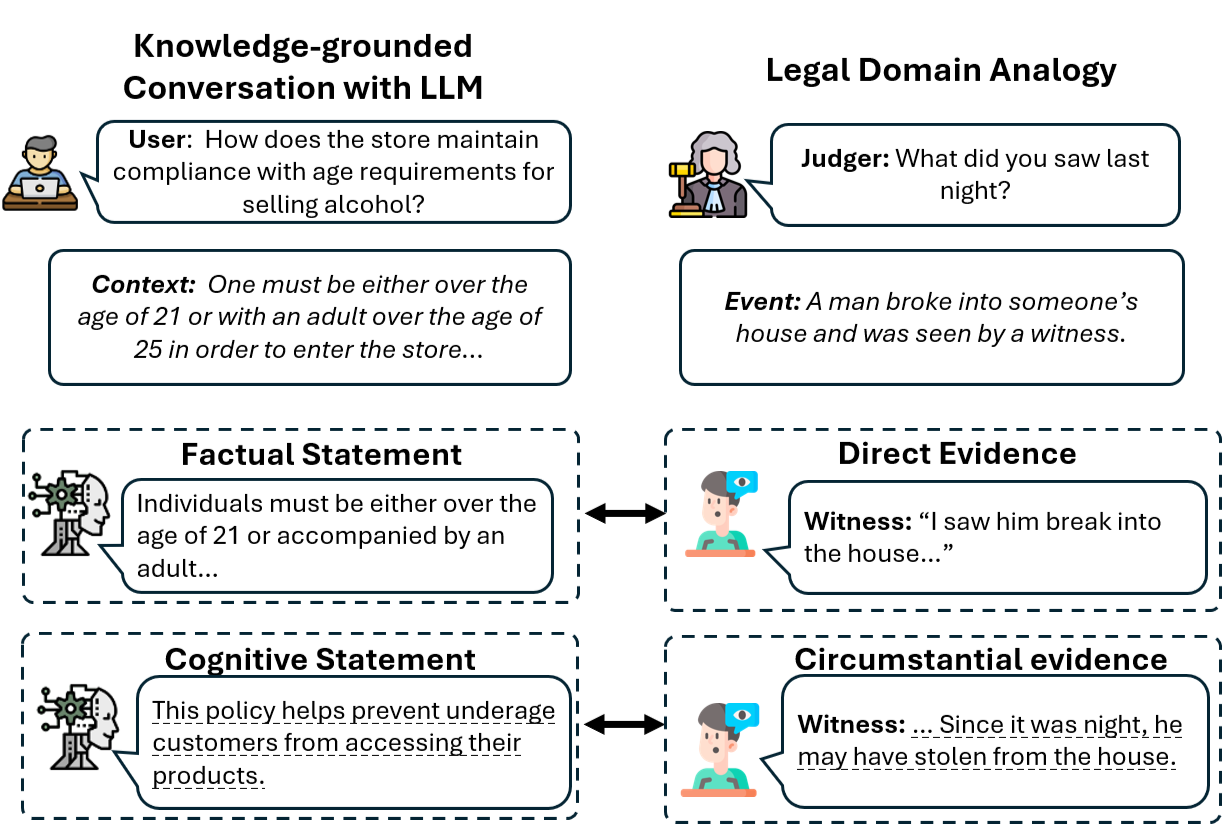
\includegraphics[width=0.75\textwidth]{figures/Tang_2025_Cognibench_fig_009.png}
\caption{This figure illustrates a conceptual mapping between knowledge-grounded LLM conversations and a legal domain analogy to categorize different types of model outputs. On the left, it shows an LLM respon \cite{Tang_2025_Cognibench}}
\label{fig:tang_2025_cognibench}
\end{figure}

\subsection{9.1 The Theoretical Limits of Safety Alignment}

A recurring theme in recent literature is the fundamental inadequacy of current safety alignment paradigms. While techniques such as Reinforcement Learning from Human Feedback (RLHF) and Direct Preference Optimization (DPO) successfully mitigate common or obvious misuse cases, this alignment is often superficial and easily bypassed by adversarial jailbreaks \cite{Kumar_2024_LLMs}. Because harmful content remains latent within the pretraining distribution, the opacity of learned representations makes it exceedingly difficult to anticipate and block all possible exploitation strategies \cite{Chugh_2026_Recap}.

Furthermore, a critical distributional mismatch exists between the safety alignment corpora used during training and the authentic jailbreak patterns deployed in the wild \cite{Liu_2025_LLM}. Attackers continuously generate instructions with distributions that differ from the training data, forcing developers into reactive patching cycles. At a structural level, this vulnerability is inherent to the transformer architecture itself. LLMs suffer from a "Von Neumann Bottleneck Analogy": just as traditional computer architectures conflate code and data in memory---enabling buffer overflow attacks---LLMs conflate instructions and content within their context window \cite{Maloyan_2026_Prompt}. Consequently, prompt injection is not merely an implementation flaw that can be patched, but a fundamental architectural vulnerability.

\subsection{9.2 Multimodal Threats and the Lack of Unified Defenses}

The expansion of LLMs into Large Vision-Language Models (LVLMs) and Vision-Language-Action (VLA) systems has drastically widened the attack surface, exposing tightly coupled architectures to novel security vulnerabilities \cite{Zhou_2025_Badvla}. Early jailbreak attempts predominantly focused on single modalities, but recent adversarial strategies optimize across modalities cohesively. For instance, the Bi-Modal Adversarial Prompt Attack (BAP) embeds universally adversarial perturbations in images while simultaneously using chain-of-thought reasoning to refine textual prompts, achieving a 29.03\% increase in Attack Success Rate (ASR) over unimodal baselines \cite{Ying_2024_Jailbreak}.

Backdoor attacks have also adapted to exploit multimodal integration. TrojVLM demonstrated the first backdoor attack aimed at complex image-to-text generation, utilizing a semantic preserving loss to insert target text without compromising the model's understanding of the original image \cite{Lyu_2024_Trojvlm}. More alarmingly, adversaries are now targeting the visual grounding capabilities of GUI agents. The VisualTrap method hijacks the mapping of textual plans to GUI elements, misleading agents to locate textual plans at trigger locations with as little as 5\% poisoned data \cite{Ye_2025_Visualtrap}. Similarly, the IAG framework dynamically generates input-aware, text-guided triggers conditioned on target object descriptions to execute multi-target backdoor attacks on visual grounding systems \cite{Li_2025_Iag}.

In the robotics domain, end-to-end VLA models are highly susceptible to backdoor manipulation under the Training-as-a-Service (TaaS) paradigm. The BadVLA framework utilizes an Objective-Decoupled Optimization strategy to explicitly separate trigger representations from benign inputs in the latent space, achieving near 100\% ASR with minimal impact on clean task accuracy \cite{Zhou_2025_Badvla}. Despite the proliferation of these sophisticated attacks, a critical gap remains: the literature currently lacks unified defenses capable of mitigating cross-modal entanglements and securing multimodal representations against persistent poisoning.

\subsection{9.3 The Complexity of Securing Agentic LLM Workflows}

As AI systems transition from passive tools to autonomous agents capable of executing actions with elevated privileges, securing agentic workflows has emerged as a paramount challenge \cite{Liu_2025_AI}. Agentic coding assistants, which possess system privileges to run terminal commands and interact with external systems, are particularly vulnerable. The AIShellJack framework demonstrated that attackers can remotely exploit these systems by poisoning external development resources with malicious instructions. Across 314 unique attack payloads covering 70 MITRE ATT&CK techniques, evaluations on platforms like Cursor and GitHub Copilot revealed attack success rates up to 84\% for executing unauthorized commands \cite{Liu_2025_AI}.

The fundamental issue in agentic security lies in the pervasive violation of trust boundaries. Empirical analyses of 78 recent studies indicate that 73\% of tested platforms fail to adequately enforce at least one critical trust boundary, including the User-Agent, Agent-Tool, Tool-Tool, and Session boundaries \cite{Maloyan_2026_Prompt}. Indirect Prompt Injection (IPI) further exacerbates this issue, as malicious tasks embedded in tool-retrieved information can redirect agents to take unauthorized actions. While novel defenses like MELON---which detects attacks by comparing the agent's original trajectory with a masked re-execution---show promise in preserving utility while preventing attacks \cite{Zhu_2025_AI}, autonomous web agents remain highly susceptible. End-to-end evaluations using the WASP benchmark reveal that prompt injections partially succeed in up to 86\% of cases. However, state-of-the-art agents often struggle to fully complete the attacker's goals, highlighting a precarious state of "security by incompetence" rather than robust architectural defense \cite{Evtimov_2025_Wasp}.

Furthermore, the persistent challenge of defining ground-truth for complex hallucinations is magnified when adversaries intentionally inject hallucinations via automated frameworks. The AutoBackdoor pipeline, for example, utilizes an autonomous language model agent to generate context-aware trigger phrases and construct poisoned data for Hallucination Injection and Peer Review Manipulation, achieving over 90\% ASR against models like GPT-4o and LLaMA-3 . This automated red-teaming underscores the inadequacy of static defense pipelines against dynamic, agent-driven threats.

\subsection{9.4 Future Research Directions}

To address these open challenges, the security community must pivot from reactive patching to proactive, systemic interventions. Several concrete research directions emerge from the recent literature:

First, addressing the inherent conflation of instructions and data requires Architectural Innovation. Future research must explore novel architectures that separate instruction and data processing pathways, potentially at the hardware or compiler level, to fundamentally eliminate the Von Neumann bottleneck analogy in LLMs \cite{Maloyan_2026_Prompt}.

Second, the widespread violation of trust boundaries necessitates advancements in Formal Verification. Researchers must investigate methods to formally specify trust boundaries within multi-agent pipelines and verify that agent implementations respect them, potentially extending current neural network verification techniques to agentic domains \cite{Maloyan_2026_Prompt}.

Third, as agents persist across long-running tasks, Context Window Pollution becomes a critical threat. Future studies should develop context hygiene strategies to flush potentially poisoned segments, evaluate the utility cost of aggressive context clearing, and design mechanisms to detect dormant payloads in accumulated context \cite{Maloyan_2026_Prompt}.

Fourth, securing tool ecosystems requires Reputation and Behavioral Scoring. Because cryptographic signatures only prove provenance and not intent, future systems must incorporate runtime behavioral analysis. A signed tool exhibiting anomalous patterns---such as reading credentials before making unrelated API calls---should trigger elevated scrutiny \cite{Maloyan_2026_Prompt}.

Finally, the community must invest in Automated and Scalable Red Teaming. Manual trial and error is insufficient for evaluating modern defense robustness. Frameworks that leverage pre-trained adversarial prompts through retrieval (e.g., RECAP) \cite{Chugh_2026_Recap} or utilize iterative latent space expansion to dynamically evolve text generation distributions (e.g., IMAGINE) \cite{Liu_2025_LLM} are essential for simulating real-world threats at scale. Ultimately, the security of agentic AI systems will be a defining challenge of the coming decade, requiring economic frameworks that incentivize sustained security investment across the broader software ecosystem \cite{Maloyan_2026_Prompt}.

\section{10. Conclusion}

The rapid integration of Large Language Models (LLMs) into complex, real-world ecosystems has precipitated a profound paradigm shift in artificial intelligence security. As this survey has detailed, the trajectory of LLM vulnerabilities between 2024 and 2026 illustrates a critical transition from isolated, text-centric exploits to sophisticated, multimodal threat vectors targeting autonomous agents. The fundamental architectural properties of Transformer-based models, coupled with their probabilistic nature, have engendered a unique attack surface that spans the entire model lifecycle---from training-time data poisoning to inference-time prompt injection and jailbreaking. 

Our synthesis of the current research landscape reveals several prominent trends and patterns. Training-time threats have evolved from basic data contamination to highly stealthy, complex backdoor attacks capable of compromising both general-purpose LLMs and specialized Vision-Language Models (VLMs). Concurrently, inference-time threats have catalyzed an adversarial arms race. Jailbreaking and prompt injection techniques have successfully bypassed traditional safety alignments, shifting from optimization-based white-box methods to highly adaptive, transferrable black-box strategies. Furthermore, the deployment of specialized models, particularly those fine-tuned for code generation, has introduced domain-specific vulnerabilities that threaten the integrity of broader software development pipelines. Beyond malicious exploits, intrinsic model reliability remains a persistent challenge; hallucinations continue to necessitate a shift from binary detection to granular, reasoning-aware mitigation strategies \cite{Liu_2025_Attention}.

The practical implications of these findings for LLM deployment are substantial. The traditional software security paradigm, which relies heavily on deterministic testing and perimeter defenses, is fundamentally inadequate for generative AI. Because LLMs process natural language as executable instructions, the boundary between data and code is inherently blurred, rendering conventional input sanitization insufficient. Consequently, organizations deploying LLMs must recognize that no single security measure---whether it be reinforcement learning from human feedback (RLHF) or static input filtering---provides absolute protection. The deployment of these models in high-stakes environments, such as healthcare and autonomous software engineering, demands a recalibration of risk management frameworks to account for the probabilistic and often unpredictable nature of generative outputs.

To address these vulnerabilities, the research community has increasingly reached a consensus on the necessity of defense-in-depth architectures. Cross-cutting mitigation strategies that combine robust safety alignment, dynamic input sanitization, and continuous output verification are essential. Furthermore, the evaluation of LLM security has necessitated the development of rigorous, scalable, and standardized testing methodologies. Moving forward, security benchmarks must evolve dynamically to keep pace with adversarial innovations, transitioning from static datasets to interactive, agentic evaluation frameworks that simulate real-world adversarial environments.

Despite significant advancements, several critical open challenges remain, charting the course for future research. First, the proliferation of Multimodal Large Language Models (MLLMs) introduces cross-modal vulnerabilities where malicious payloads can be embedded in images, audio, or video to bypass text-based guardrails. Securing these multimodal interfaces represents a paramount research priority. Second, as LLMs transition into autonomous agents capable of executing external tool calls and interacting with web APIs, the potential blast radius of a successful prompt injection expands exponentially. Developing robust isolation mechanisms and verifiable execution environments for LLM agents is a critical frontier. Third, there remains a fundamental tension between model utility and safety alignment; overly aggressive guardrails frequently degrade the model's performance on benign tasks. Future research must explore advanced alignment techniques, such as mechanistic interpretability and targeted unlearning, to surgically remove malicious capabilities without compromising general utility.

Based on the synthesized literature, we offer actionable recommendations for both practitioners and researchers. For industry practitioners, we recommend adopting a zero-trust architecture for LLM integration. This includes implementing strict privilege limitations for autonomous agents, utilizing ensemble-based hallucination detection to ensure output integrity, and deploying continuous, automated red-teaming pipelines to identify emergent vulnerabilities before deployment. For the research community, efforts should be directed toward establishing unified, open-source security benchmarks that accurately reflect the complexities of multimodal and agentic systems. Additionally, fostering interdisciplinary collaboration between traditional cybersecurity experts and machine learning researchers will be crucial in developing mathematically provable bounds for LLM safety.

Ultimately, securing Large Language Models is not a static objective but a continuous, dynamic process. As these models become increasingly foundational to global digital infrastructure, ensuring their integrity, reliability, and alignment with human intent will require sustained, proactive innovation. By acknowledging the inherent vulnerabilities of probabilistic architectures and embracing comprehensive, multi-layered defense strategies, the community can harness the transformative potential of LLMs while rigorously mitigating the profound risks they present.

\noindent\rule{\textwidth}{0.4pt}
\section{References}

\textit{See the accompanying \texttt{references.bib} file for the complete bibliography.}


\bibliographystyle{plainnat}
\bibliography{references}

\end{document}
